%%%%%% Run at command line, run
%%%%%% xelatex grad-sample.tex 
%%%%%% for a few times to generate the output pdf file
\documentclass[12pt,oneside,openright,a4paper]{cpe-thai-project}


\usepackage{polyglossia}
\usepackage{enumitem,lipsum}
\usepackage{graphicx}
\usepackage{placeins}

\usepackage{multirow}
\usepackage{colortbl}
\usepackage{graphicx}
\usepackage[table,xcdraw]{xcolor}

\graphicspath{ {./images/} }
\setdefaultlanguage{thai}
\setotherlanguage{english}
\newfontfamily\thaifont[Script=Thai,Scale=1.23]{TH Sarabun New}
\defaultfontfeatures{Mapping=tex-text,Scale=1.23,LetterSpace=0.0}
\setmainfont[Scale=1.23,LetterSpace=0,WordSpace=1.0,FakeStretch=1.0,Mapping=tex-text]{TH Sarabun New}
\XeTeXlinebreaklocale "th"	
\XeTeXlinebreakskip = 0pt plus 0pt
\emergencystretch=10pt

%%%%%%%%%%%%%%%%%%%%%%%%%%%%%%%%%%%%%%%%%%%%%%%%%%%%%%%%%%%%%%%%%%%
% Customize below to suit your needs 
% The ones that are optional can be left blank. 
%%%%%%%%%%%%%%%%%%%%%%%%%%%%%%%%%%%%%%%%%%%%%%%%%%%%%%%%%%%%%%%%%%%
% First line of title
\def\disstitleone{Will Chain }   
% Second line of title
\def\disstitletwo{Will On Blockchain}   
% Your first name and lastname
\def\dissauthor{MR. THITIPONG BOONTHANAKORN}   % 1st member
%%% Put other group member names here ..
\def\dissauthortwo{MR. NARONGYOT SOONTHARARAK}   % 2nd member (optional)
\def\dissauthorthree{MR. SUBTAWEE NGANRUNGRUANG}   % 3rd member (optional)


% The degree that you're persuing..
\def\dissdegree{Bachelor of Engineering} % Name of the degree
\def\dissdegreeabrev{B.Eng} % Abbreviation of the degree
\def\dissyear{2022}                   % Year of submission
\def\thaidissyear{2565}               % Year of submission (B.E.)

%%%%%%%%%%%%%%%%%%%%%%%%%%%%%%%%%%%%%%%%%%%%
% Your project and independent study committee..
%%%%%%%%%%%%%%%%%%%%%%%%%%%%%%%%%%%%%%%%%%%%
\def\dissadvisor{Asst.Prof. Marong Phadoongsidhi, Ph.D.}  % Advisor
%%% Leave it empty if you have no Co-advisor
\def\disscoadvisor{}  % Co-advisor
\def\disscommitteetwo{Mrs. Piyanit Wepulanon , Ph.D.}  % 3rd committee member (optional)
\def\disscommitteethree{Asst.Prof. Thumrongrat Amornraksa , Ph.D.}
\def\disscommitteefour{Asst.Prof. Surapont Toomnark}    % 5th committee member (optional) 

\def\worktype{Project} %%  Project or Independent study
\def\disscredit{3}   %% 3 credits or 6 credits


\def\fieldofstudy{Computer Engineering} 
\def\department{Computer Engineering} 
\def\faculty{Engineering}

\def\thaifieldofstudy{วิศวกรรมคอมพิวเตอร์} 
\def\thaidepartment{วิศวกรรมคอมพิวเตอร์} 
\def\thaifaculty{วิศวกรรมศาสตร์}
 
\def\appendixnames{Appendix} %%% Appendices or Appendix

\def\thaiworktype{ปริญญานิพนธ์} %  Project or research project % 
\def\thaidisstitleone{Will Chain}
\def\thaidisstitletwo{Will on Blockchain}
\def\thaidissauthor{นายฐิติพงศ์ บุณธนากร}
\def\thaidissauthortwo{นายณรงค์ยศ สุนทรารักษ์} %Optional
\def\thaidissauthorthree{นายทรัพย์ทวี งานรุ่งเรือง} %Optional

\def\thaidissadvisor{ผศ.ดร.มารอง ผดุงสิทธิ์}
%% Leave this empty if you have no co-advisor
\def\thaidisscoadvisor{รศ.ดร.ที่ปรึกษา วิทยานิพนธ์ร่วม} %Optional
\def\thaidissdegree{วิศวกรรมศาสตรบัณฑิต}

% Change the line spacing here...
\linespread{1.15}

%%%%%%%%%%%%%%%%%%%%%%%%%%%%%%%%%%%%%%%%%%%%%%%%%%%%%%%%%%%%%%%%
% End of personal customization.  Do not modify from this part 
% to \begin{document} unless you know what you are doing...
%%%%%%%%%%%%%%%%%%%%%%%%%%%%%%%%%%%%%%%%%%%%%%%%%%%%%%%%%%%%%%%%


%%%%%%%%%%%% Dissertation style %%%%%%%%%%%
%\linespread{1.6} % Double-spaced  
%%\oddsidemargin    0.5in
%%\evensidemargin   0.5in
%%%%%%%%%%%%%%%%%%%%%%%%%%%%%%%%%%%%%%%%%%%
%\renewcommand{\subfigtopskip}{10pt}
%\renewcommand{\subfigbottomskip}{-5pt} 
%\renewcommand{\subfigcapskip}{-6pt} %vertical space between caption
%                                    %and figure.
%\renewcommand{\subfigcapmargin}{0pt}

\renewcommand{\topfraction}{0.85}
\renewcommand{\textfraction}{0.1}

\newtheorem{theorem}{Theorem}
\newtheorem{lemma}{Lemma}
\newtheorem{corollary}{Corollary}

\def\QED{\mbox{\rule[0pt]{1.5ex}{1.5ex}}}
\def\proof{\noindent\hspace{2em}{\itshape Proof: }}
\def\endproof{\hspace*{\fill}~\QED\par\endtrivlist\unskip}
%\newenvironment{proof}{{\sc Proof:}}{~\hfill \blacksquare}
%% The hyperref package redefines the \appendix. This one 
%% is from the dissertation.cls
%\def\appendix#1{\iffirstappendix \appendixcover \firstappendixfalse \fi \chapter{#1}}
%\renewcommand{\arraystretch}{0.8}
%%%%%%%%%%%%%%%%%%%%%%%%%%%%%%%%%%%%%%%%%%%%%%%%%%%%%%%%%%%%%%%%
%%%%%%%%%%%%%%%%%%%%%%%%%%%%%%%%%%%%%%%%%%%%%%%%%%%%%%%%%%%%%%%%

\usepackage{ragged2e}
\begin{document}

\pdfstringdefDisableCommands{%
\let\MakeUppercase\relax
}

\begin{center}
  
\includegraphics[width=2.8cm]{logo02.jpg}
\end{center}
\vspace*{-1cm}

\maketitlepage
\makesignaturepage 

%%%%%%%%%%%%%%%%%%%%%%%%%%%%%%%%%%%%%%%%%%%%%%%%%%%%%%%%%%%%%%
%%%%%%%%%%%%%%%%%%%%%% English abstract %%%%%%%%%%%%%%%%%%%%%%%
%%%%%%%%%%%%%%%%%%%%%%%%%%%%%%%%%%%%%%%%%%%%%%%%%%%%%%%%%%%%%%
\abstract

Will Chain is a platform developed with the aim of studying how Blockchain networks work and managing wills in real-world assets. and digital assets. Will Chain will include features for managing and keeping current wills. that can meet both real-life assets and digital assets There will be a feature that will support the addition of a will, namely a feature for delivering assets to heirs. If the conditions are the same as in the will Makes wills more secure because the system will not go through the hands of an intermediary but will only have that system. It is also convenient to make wills. and will have even greater coverage.

\begin{flushleft}
\begin{tabular*}{\textwidth}{@{}lp{0.8\textwidth}}
\textbf{Keywords}: & Asset / Blockchain / Cryptocurrency / Digital Asset / Finance / Non-Fungible Token(NFT) /  Smart Contract / Will 
\end{tabular*}
\end{flushleft}
\endabstract

%%%%%%%%%%%%%%%%%%%%%%%%%%%%%%%%%%%%%%%%%%%%%%%%%%%%%%%%%%%%%%
%%%%%%%%%% Thai abstract here %%%%%%%%%%%%%%%%%%%%%%%%%%%%%%%%%
%%%%%%%%%%%%%%%%%%%%%%%%%%%%%%%%%%%%%%%%%%%%%%%%%%%%%%%%%%%%%%
% {\newfontfamily\thaifont{TH Sarabun New:script=thai}[Scale=1.3]
% \XeTeXlinebreaklocale "th_TH"	
% \thaifont
\newcommand\tab[1][1cm]{\hspace*{#1}}
\thaiabstract

\tab Will Chain เป็นแพลตฟอร์มที่ถูกพัฒนาขึ้นมาโดยมีวัตถุประสงค์เพื่อศึกษาการทำงานของเครือข่าย Blockchain  และจัดการเกี่ยวกับพินัยกรรมในด้านของสินทรัพย์ในโลกความเป็นจริง และสินทรัพย์ดิจิทัล โดยที่ Will Chain นั้นจะมีฟีเจอร์ในการจัดการและเก็บรักษาพินัยกรรมที่มีอยู่ในปัจจุบัน ที่จะสามารถตอบโจทย์ได้ทั้งสินทรัพย์ในชีวิตจริงและสินทรัพย์ดิจิทัล โดยจะมีฟีเจอร์ที่จะรองรับการทำพินัยกรรมเพิ่มเติมคือฟีเจอร์สำหรับการส่งมอบสินทรัพย์ให้กับทายาท ถ้ามีเงื่อนไขตรงกับในพินัยกรรม ทำให้การทำพินัยกรรมนั้นมีความปลอดภัยมากขึ้นเนื่องจากตัวระบบจะไม่ผ่านมือคนกลางแต่จะมีแค่ระบบนั้น อีกทั้งสะดวกในการทำพินัยกรรม และจะมีความครอบคลุมที่มากยิ่งขึ้น
\begin{flushleft}
\begin{tabular*}{\textwidth}{@{}lp{0.8\textwidth}}
 & \\

\textbf{คำสำคัญ}: & Asset / Blockchain / Cryptocurrency / Digital Asset / Finance / Non-Fungible Token(NFT) /  Smart Contract / Will 
\end{tabular*}
\end{flushleft}
\endabstract

%}

%%%%%%%%%%%%%%%%%%%%%%%%%%%%%%%%%%%%%%%%%%%%%%%%%%%%%%%%%%%%
%%%%%%%%%%%%%%%%%%%%%%% Acknowledgments %%%%%%%%%%%%%%%%%%%%
%%%%%%%%%%%%%%%%%%%%%%%%%%%%%%%%%%%%%%%%%%%%%%%%%%%%%%%%%%%%
\preface
\tab การทําโครงงานครั้งนี้สําเร็จลงได้ด้วยความช่วยเหลือของ ผู้ช่วยศาสตราจารย์ ดร. มารอง ผดุงสิทธิ์ ที่ปรึกษาโครงงาน ซึ่งได้ให้ความกรุณา สละเวลาให้คําปรึกษา คําแนะนํา ข้อเสนอแนะอันมีประโยชน์อย่างมาก และความช่วยเหลือตลอดการทําโครงงานนี้จนสําเร็จลุล่วงได้ด้วยดี ผู้จัดทําโครงงานจึงขอกราบขอบพระคุณเป็นอย่างสูง

\tab ขอขอบพระคุณ ผ.ศ.สุรพนธ์ ตุ้มนาค , ดร.ปิยนิตย์ เวปุลานนท์ และ รศ.ดร.ธํารงรัตน์ อมรรักษา ที่ได้สละเวลา
ร่วมเป็นคณะกรรมการตรวจสอบโครงงานในครั้งนี้ 

\tab ท้ายที่สุดนี้ โครงงานนี้อาจจะไม่สําเร็จเลยหากไม่มีเพื่อนในภาควิชาวิศวกรรมคอมพิวเตอร์ มหาวิทยาลัยเทคโนโลยีพระจอมเกล้าธนบุรีที่ให้ 
ความช่วยเหลือ การสนับสนุน รวมทั้งคอยเป็นกําลังใจสําคัญเสมอมา 

\tab ทีมผู้จัดทำหวังว่าโครงงานนี้จะก่อให้เกิดประโยชน์ต่อการทำพินัยกรรมในปัจจุบัน และสามารถครอบคลุมไปถึงพินัยกรรมของสินทรัพย์ดิจิทัลที่ยังไม่มีเทคโนโลยีรองรับในตอนนี้ และเกิดการเปลี่ยนแปลงที่ดีขึ้นในอนาคต

%%%%%%%%%%%%%%%%%%%%%%%%%%%%%%%%%%%%%%%%%%%%%%%%%%%%%%%%%%%%%
%%%%%%%%%%%%%%%% ToC, List of figures/tables %%%%%%%%%%%%%%%%
%%%%%%%%%%%%%%%%%%%%%%%%%%%%%%%%%%%%%%%%%%%%%%%%%%%%%%%%%%%%%
% The three commands below automatically generate the table 
% of content, list of tables and list of figures
\tableofcontents                    
\listoftables
\listoffigures                      

%%%%%%%%%%%%%%%%%%%%%%%%%%%%%%%%%%%%%%%%%%%%%%%%%%%%%%%%%%%%%%
%%%%%%%%%%%%%%%%%%%%% List of symbols page %%%%%%%%%%%%%%%%%%%
%%%%%%%%%%%%%%%%%%%%%%%%%%%%%%%%%%%%%%%%%%%%%%%%%%%%%%%%%%%%%%
% You have to add this manually..
\listofsymbols
\begin{flushleft}
\begin{tabular}{@{}p{0.07\textwidth}p{0.7\textwidth}p{0.1\textwidth}}
\textbf{SYMBOL}  & & \textbf{UNIT} \\[0.2cm]
$\alpha$ & Test variable\hfill & m$^2$ \\
$\lambda$ & Interarival rate\hfill &  jobs/second\\
$\mu$ & Service rate\hfill & jobs/second\\
\end{tabular}
\end{flushleft}
%%%%%%%%%%%%%%%%%%%%%%%%%%%%%%%%%%%%%%%%%%%%%%%%%%%%%%%%%%%%%%
%%%%%%%%%%%%%%%%%%%%% List of vocabs & terms %%%%%%%%%%%%%%%%%
%%%%%%%%%%%%%%%%%%%%%%%%%%%%%%%%%%%%%%%%%%%%%%%%%%%%%%%%%%%%%%
% You also have to add this manually..
\listofvocab
\begin{flushleft}
\begin{tabular}{@{}p{1in}@{=\extracolsep{0.5in}}l}
Asset & ทรัพย์สินที่เรามีอยู่ทั้งหมด  เงินที่อยู่ในบัญชีทั้งหมดอยู่ในกระเป๋าทั้งหมดรวมทั้งหนี้สินที่เรามีอยู่ทั้งหมด \\
Blockchain & ระบบโครงข่ายในการเก็บบัญชีธุรกรรมออนไลน์ \\
Cryptocurrency & สกุลเงินเข้ารหัส เป็นสินทรัพย์ดิจิทัล \\
Digital Asset & สิ่งที่มีมูลค่าและเราสามารถเป็นเจ้าของได้ แต่ไม่สามารถแตะต้องได้ทางกายภาพ\\
Finance & การเงิน\\
Non-Fungible Token(NFT) & สิ่งของที่มีความแตกต่างเฉพาะตัวไม่สามารถทดแทนกันได้หรือซื้อเป็นหน่วยย่อยได้\\
Smart Contract & กระบวนการทางดิจิทัล ที่กำหนดขั้นตอนการทำธุรกรรมโดยอัตโนมัติไว้ล่วงหน้า โดยไม่ต้องอาศัยตัวกลาง\\
Will  & คือพินัยกรรมที่เก็บคำสั่งเสียสุดท้ายในการทำกิจการต่าง ๆ \\
\end{tabular}
\end{flushleft}

%\setlength{\parskip}{1.2mm}

%%%%%%%%%%%%%%%%%%%%%%%%%%%%%%%%%%%%%%%%%%%%%%%%%%%%%%%%%%%%%%%
%%%%%%%%%%%%%%%%%%%%%%%% Main body %%%%%%%%%%%%%%%%%%%%%%%%%%%%
%%%%%%%%%%%%%%%%%%%%%%%%%%%%%%%%%%%%%%%%%%%%%%%%%%%%%%%%%%%%%%%


\chapter{บทนำ}

\section{ที่มาและความสำคัญ}

\tab ในปัจจุบันนั้นเทคโนโลยีเข้ามามีบทบาทในการใช้ชีวิตของผู้คนเป็นอย่างมาก ไม่ว่าจะเป็นในด้านของ การเงิน สินทรัพย์ เป็นต้น แต่ว่าจะมีในด้านของพินัยกรรมที่นับว่าเป็นเอกสารที่ไม่มีการใช้เทคโนโลยีเข้ามาช่วยเหลือในปัจจุบัน โดยยังที่จะต้องทำการเก็บรักษาไว้ที่ตัวเองหรือไม่ก็เก็บไว้ที่ทนายของตนเองทำให้บางครั้งพินัยกรรมนั้น ๆ อาจเกิดการเสียหายหรือสูญหายได้ หรือแม้กระทั่งอาจเกิดโอกาสเปลี่ยนแปลงจากบุคคลที่สามได้ ทำให้การทำพินัยกรรมในแต่ละครั้งมีความยุ่งยากและไม่ปลอดภัยสำหรับผู้ที่จะทำพินัยกรรม รวมถึงพินัยกรรมในส่วนนี้ยังครอบคลุมในด้านของการสืบทอดสินทรัพย์ดิจิทัล อย่างเช่น Cryptocurrency ได้ เนื่องจากยังไม่มีเทคโนโลยีที่รองรับในปัจจุบัน

\tab จึงเกิดแนวคิดที่จะสร้าง แพลตฟอร์มสำหรับจัดการพินัยกรรมทั้งสินทรัพย์ในโลกความเป็นจริง และสินทรัพย์ดิจิทัลผ่านระบบ Blockchain\ ที่สามารถนำพินัยกรรมที่มีอยู่ในปัจจุบันนั้นเอาขึ้นระบบ Blockchain เพื่อเก็บรักษาพินัยกรรมนั้น และสามารถทำการสืบทอดสินทรัพย์ไปยังผู้รับพินัยกรรมได้ รวมไปถึงสินทรัพย์ดิจิทัลอีกด้วย โดยคำนึงถึงความปลอดภัยและความสะดวกสบายของผู้ใช้งาน


\section{วัตถุประสงค์}

\begin{itemize}
\item เพื่อศึกษาเทคโนโลยี Blockchain
\item เพื่อสร้างแพลตฟอร์มสำหรับจัดการพินัยกรรมทั้งสินทรัพย์ในโลกความเป็นจริง และสินทรัพย์ดิจิทัล
\item เพื่อให้พินัยกรรมในปัจจุบันสามารถครอบคลุมถึงสินทรัพย์ดิจิทัล
\item เพื่อเก็บรักษาพินัยกรรมให้มีความปลอดภัยมากขึ้น
\item เพื่ออำนวยความสะดวกในการเก็บพินัยกรรม
\end{itemize}

\section{ขอบเขตของโครงงาน}

\begin{itemize}
\item พัฒนาแพลตฟอร์มสำหรับจัดการพินัยกรรมทั้งสินทรัพย์ในโลกความเป็นจริง และสินทรัพย์ดิจิทัล
\item ใช้ภาษา Solidity ในการพัฒนา Smart Contract
\end{itemize}

\section{ประโยชน์ที่คาดว่าจะได้่รับ}
\tab Will Chain เป็นการใช้เทคโนโลยี Blockchain เพื่อการทำพินัยกรรมโดยจะสามารถถ่ายทอดมรดกที่เป็นสินทรัพย์ที่ระบบรองรับจากผู้ที่ทำการเขียนพินัยกรรม ไปหาผู้รับสินทรัพย์ได้ด้วยรูปแบบของ NFT หรือ F-NFT
\section{เนื้อหาทางวิศวกรรมที่เป็นต้นฉบับ}
\tab โครงงานนี้พัฒนาขึ้นมาจากการใช้ความรู้ในด้าน Blockchain Technology (Ethereum chain โดยใช้เครื่องมือพัฒนา Smart Contract ด้วยภาษา Solidity ในการพัฒนา)  และใช้ความรู้เรื่อง NFT , F-NFT เพื่อใช้ในการเก็บข้อมูลพินัยกรรมของตัวโปรเจคของเรา รวมถึงการทำ Decentralize  Application ที่ใช้ Next Typescript Framework ในการพัฒนาส่วนติดต่อกับผู้ใช้รวมไปถึงความรู้ด้าน วิศวกรรมซอฟแวร์ และ ด้านพินัยกรรม เพื่อที่จะสามารถทำการถ่ายทอดพินัยกรรมได้ภายใน Decentralize  Application
\section{การแยกย่อยงาน และร่างแผนคำแนะนำจากอาจารย์ที่ปรึกษา}
\begin{enumerate}
\item ศึกษาค้นคว้าที่มาและความสำคัญของปัญหา
\item เสนอหัวข้อโครงการให้กับอาจารย์ที่ปรึกษา
\item ทำการสำรวจหรือศึกษาค้นคว้าข้อมูลที่เกี่ยวข้องกับโครงงาน
	\begin{itemize}
		\item ศึกษาเรื่องพินัยกรรม
		\item ศึกษาเรื่องกฎหมาย
		\item ศึกษาเรื่องสินทรัพย์
	\end{itemize}
\item นำเสนอโครงการและข้อมูลทึ่ศึกษาค้นคว้าให้กับอาจารย์ที่ปรึกษา
\item จัดทำข้อเสนอโครงการ
\item นำเสนอข้อเสนอโครงการ
\item จัดทำรายงาน
	\begin{itemize}
		\item รายงานบทที่ 1 จากข้อมูลข้อเสนอโครงงาน
		\item รายงานบทที่ 2 จากข้อมูลการศึกษาค้นคว้าเกี่ยวกับทฤษฎีที่เกี่ยวข้อง
		\item รายงานบทที่ 3 รายงานการออกแบบการทำงานของระบบเบื้องต้น
	\end{itemize}
\item วิเคราะห์และออกแบบระบบ
	\begin{itemize}
		\item ออกแบบการทำงาน Algorithms ของ Smart Contract ที่ใช้งานในระบบ
		\item ออกแบบรูปแบบพินัยกรรมที่จะใช้ในระบบ
		\item ออกแบบส่วนของผู้ใช้งาน (UX/UI)
	\end{itemize}
\item ศึกษาและพัฒนา Blockchain และ Smart Contract
	\begin{itemize}
		\item ศึกษาการทำงานของ Blockchain ด้วย Ethereum chain
		\item ศึกษาและพัฒนาส่วนของ Smart Contract ที่ใช้ในการควบคุมระบบด้วยภาษา Solidity
		\item ศึกษาและพัฒนา NFT ในระบบ
	\end{itemize}
\item ศึกษาและพัฒนา Web application
	\begin{itemize}
		\item ศึกษาและพัฒนาส่วนของผู้ใช้งานด้วย Next.js Typescript และ User Interface Framework อื่น ๆ 
		\item ศึกษาเกี่ยวกับ API ของหน่วยงานรัฐ
	\end{itemize}
\item นำเสนอโครงงาน 3 บท
\item ศึกษาและพัฒนา Blockchain และ Smart Contract (ต่อจากภาคการศึกษาที่ 1)
\item ทดสอบการทำงานของ Ethereum chain
\item ปรับปรุงและแก้ไข Ethereum chain
\item ศึกษาและพัฒนา Web application (ต่อจากภาคการศึกษาที่ 1)
\item ทดสอบการทำงานของ Web application
\item ปรับปรุงและแก้ไข Web application
\item จัดทำรายงงานโครงงานฉบับสมบูรณ์
\item นำเสนอโครงงาน
\end{enumerate}

\section{ตารางการดำเนินงาน}

\begin{table}
\centering
\caption{ตารางการดำเนินงาน ประจำภาคการศึกษาที่ 1/2565}
\resizebox{\linewidth}{!}{%
\begin{tabular}{|l|l|l|l|l|l|l|l|l|l|l|l|l|l|l|l|l|l|l|l|l|l|} 
\hline
\multicolumn{22}{|c|}{ตารางการดำเนินงาน ประจำภาคการศึกษาที่ 1/2565}                                                                                                                                                                                                                                                                                                                                                                                                                                                                                                                                                                                                                                                                                                                                                                                                                                                   \\ 
\hline
\multicolumn{1}{|c|}{\multirow{3}{*}{ที่}} & \multicolumn{1}{c|}{\multirow{3}{*}{หัวข้อการดำเนินงาน}}    & \multicolumn{20}{c|}{ระยะเวลา}                                                                                                                                                                                                                                                                                                                                                                                                                                                                                                                                                                                                                                                                                                                                                                             \\ 
\cline{3-22}
\multicolumn{1}{|c|}{}                     & \multicolumn{1}{c|}{}                                       & \multicolumn{4}{c|}{สิงหาคม}                                                                                                                              & \multicolumn{4}{c|}{กันยายน}                                                                                                                              & \multicolumn{4}{c|}{ตุลาคม}                                                                                                                               & \multicolumn{4}{c|}{พฤศจิกายน}                                                                                                                            & \multicolumn{4}{c|}{ธันวาคม}                                                                                                                               \\ 
\cline{3-22}
\multicolumn{1}{|c|}{}                     & \multicolumn{1}{c|}{}                                       & \multicolumn{1}{c|}{1}               & \multicolumn{1}{c|}{2}               & \multicolumn{1}{c|}{3}               & \multicolumn{1}{c|}{4}               & \multicolumn{1}{c|}{1}               & \multicolumn{1}{c|}{2}               & \multicolumn{1}{c|}{3}               & \multicolumn{1}{c|}{4}               & \multicolumn{1}{c|}{1}               & \multicolumn{1}{c|}{2}               & \multicolumn{1}{c|}{3}               & \multicolumn{1}{c|}{4}               & \multicolumn{1}{c|}{1}               & \multicolumn{1}{c|}{2}               & \multicolumn{1}{c|}{3}               & \multicolumn{1}{c|}{4}               & \multicolumn{1}{c|}{1}               & \multicolumn{1}{c|}{2}               & \multicolumn{1}{c|}{3}               & \multicolumn{1}{c|}{4}                \\ 
\hline
1                                          & ศึกษาค้นคว้าที่มาของและ ความสำคัญของปัญหา                   & {\cellcolor[rgb]{0.176,0.549,0.624}} &                                      &                                      &                                      &                                      &                                      &                                      &                                      &                                      &                                      &                                      &                                      &                                      &                                      &                                      &                                      &                                      &                                      &                                      &                                       \\ 
\hline
2                                          & เสนอหัวข้อโครงการให้กับอาจารย์
ที่ปรึกษา~ ~                 &                                      & {\cellcolor[rgb]{0.176,0.549,0.624}} &                                      &                                      &                                      &                                      &                                      &                                      &                                      &                                      &                                      &                                      &                                      &                                      &                                      &                                      &                                      &                                      &                                      &                                       \\ 
\hline
3                                          & ทำการสำรวจหรือศึกษาค้นขว้า
ข้อมูลที่เกี่ยวข้องกับโครงงาน    & {\cellcolor[rgb]{0.176,0.549,0.624}} & {\cellcolor[rgb]{0.176,0.549,0.624}} & {\cellcolor[rgb]{0.176,0.549,0.624}} & {\cellcolor[rgb]{0.176,0.549,0.624}} &                                      &                                      &                                      &                                      &                                      &                                      &                                      &                                      &                                      &                                      &                                      &                                      &                                      &                                      &                                      &                                       \\ 
\hline
4                                          & นำเสนอโครงการและข้อมูลทึ่ศึกษาค้นคว้าให้กับอาจารย์ที่ปรึกษา & {\cellcolor[rgb]{0.176,0.549,0.624}} & {\cellcolor[rgb]{0.176,0.549,0.624}} & {\cellcolor[rgb]{0.176,0.549,0.624}} & {\cellcolor[rgb]{0.176,0.549,0.624}} & {\cellcolor[rgb]{0.176,0.549,0.624}} & {\cellcolor[rgb]{0.176,0.549,0.624}} & {\cellcolor[rgb]{0.176,0.549,0.624}} & {\cellcolor[rgb]{0.176,0.549,0.624}} & {\cellcolor[rgb]{0.176,0.549,0.624}} & {\cellcolor[rgb]{0.176,0.549,0.624}} & {\cellcolor[rgb]{0.176,0.549,0.624}} & {\cellcolor[rgb]{0.176,0.549,0.624}} & {\cellcolor[rgb]{0.176,0.549,0.624}} & {\cellcolor[rgb]{0.176,0.549,0.624}} & {\cellcolor[rgb]{0.176,0.549,0.624}} & {\cellcolor[rgb]{0.176,0.549,0.624}} & {\cellcolor[rgb]{0.176,0.549,0.624}} & {\cellcolor[rgb]{0.176,0.549,0.624}} & {\cellcolor[rgb]{0.176,0.549,0.624}} & {\cellcolor[rgb]{0.176,0.549,0.624}}  \\ 
\hline
5                                          & จัดทำข้อเสนอโครงการ~ ~                                      &                                      &                                      &                                      &                                      & {\cellcolor[rgb]{0.176,0.549,0.624}} & {\cellcolor[rgb]{0.176,0.549,0.624}} &                                      &                                      &                                      &                                      &                                      &                                      &                                      &                                      &                                      &                                      &                                      &                                      &                                      &                                       \\ 
\hline
6                                          & นำเสนอข้อเสนอโครงการ                                        &                                      &                                      &                                      &                                      &                                      & {\cellcolor[rgb]{0.176,0.549,0.624}} &                                      &                                      &                                      &                                      &                                      &                                      &                                      &                                      &                                      &                                      &                                      &                                      &                                      &                                       \\ 
\hline
7                                          & จัดทำรายงาน~ ~                                              &                                      &                                      &                                      &                                      &                                      & {\cellcolor[rgb]{0.176,0.549,0.624}} & {\cellcolor[rgb]{0.176,0.549,0.624}} & {\cellcolor[rgb]{0.176,0.549,0.624}} & {\cellcolor[rgb]{0.176,0.549,0.624}} & {\cellcolor[rgb]{0.176,0.549,0.624}} & {\cellcolor[rgb]{0.176,0.549,0.624}} & {\cellcolor[rgb]{0.176,0.549,0.624}} & {\cellcolor[rgb]{0.176,0.549,0.624}} & {\cellcolor[rgb]{0.176,0.549,0.624}} & {\cellcolor[rgb]{0.176,0.549,0.624}} & {\cellcolor[rgb]{0.176,0.549,0.624}} &                                      &                                      &                                      &                                       \\ 
\hline
8                                          & วิเคราะห์และออกแบบระบบ                                      &                                      &                                      &                                      &                                      &                                      & {\cellcolor[rgb]{0.176,0.549,0.624}} & {\cellcolor[rgb]{0.176,0.549,0.624}} & {\cellcolor[rgb]{0.176,0.549,0.624}} & {\cellcolor[rgb]{0.176,0.549,0.624}} & {\cellcolor[rgb]{0.176,0.549,0.624}} & {\cellcolor[rgb]{0.176,0.549,0.624}} & {\cellcolor[rgb]{0.176,0.549,0.624}} & {\cellcolor[rgb]{0.176,0.549,0.624}} & {\cellcolor[rgb]{0.176,0.549,0.624}} & {\cellcolor[rgb]{0.176,0.549,0.624}} & {\cellcolor[rgb]{0.176,0.549,0.624}} & {\cellcolor[rgb]{0.176,0.549,0.624}} & {\cellcolor[rgb]{0.176,0.549,0.624}} & {\cellcolor[rgb]{0.176,0.549,0.624}} & {\cellcolor[rgb]{0.176,0.549,0.624}}  \\ 
\hline
9                                          & ศึกษาและพัฒนา Blockchain และ Smart Contract                 &                                      &                                      &                                      &                                      &                                      & {\cellcolor[rgb]{0.176,0.549,0.624}} & {\cellcolor[rgb]{0.176,0.549,0.624}} & {\cellcolor[rgb]{0.176,0.549,0.624}} & {\cellcolor[rgb]{0.176,0.549,0.624}} & {\cellcolor[rgb]{0.176,0.549,0.624}} & {\cellcolor[rgb]{0.176,0.549,0.624}} & {\cellcolor[rgb]{0.176,0.549,0.624}} & {\cellcolor[rgb]{0.176,0.549,0.624}} & {\cellcolor[rgb]{0.176,0.549,0.624}} & {\cellcolor[rgb]{0.176,0.549,0.624}} & {\cellcolor[rgb]{0.176,0.549,0.624}} & {\cellcolor[rgb]{0.176,0.549,0.624}} & {\cellcolor[rgb]{0.176,0.549,0.624}} & {\cellcolor[rgb]{0.176,0.549,0.624}} & {\cellcolor[rgb]{0.176,0.549,0.624}}  \\ 
\hline
10                                         & ศึกษาและพัฒนา Web application~ ~                            &                                      &                                      &                                      &                                      &                                      & {\cellcolor[rgb]{0.176,0.549,0.624}} & {\cellcolor[rgb]{0.176,0.549,0.624}} & {\cellcolor[rgb]{0.176,0.549,0.624}} & {\cellcolor[rgb]{0.176,0.549,0.624}} & {\cellcolor[rgb]{0.176,0.549,0.624}} & {\cellcolor[rgb]{0.176,0.549,0.624}} & {\cellcolor[rgb]{0.176,0.549,0.624}} & {\cellcolor[rgb]{0.176,0.549,0.624}} & {\cellcolor[rgb]{0.176,0.549,0.624}} & {\cellcolor[rgb]{0.176,0.549,0.624}} & {\cellcolor[rgb]{0.176,0.549,0.624}} & {\cellcolor[rgb]{0.176,0.549,0.624}} & {\cellcolor[rgb]{0.176,0.549,0.624}} & {\cellcolor[rgb]{0.176,0.549,0.624}} & {\cellcolor[rgb]{0.176,0.549,0.624}}  \\ 
\hline
11                                         & นำเสนอโครงงาน 3 บท                                          &                                      &                                      &                                      &                                      &                                      &                                      &                                      &                                      &                                      &                                      &                                      &                                      &                                      &                                      &                                      &                                      & {\cellcolor[rgb]{0.176,0.549,0.624}} &                                      &                                      &                                       \\
\hline
\end{tabular}
}
\end{table}

\begin{table}[]
\centering
\caption{ตารางการดําเนินงาน ประจําภาคการศึกษาที่ 2/2565}
\label{tab:my-table}
\resizebox{\textwidth}{!}{%
\begin{tabular}{|llllllllllllllllll|}
\hline
\multicolumn{18}{|c|}{ตารางการดำเนินงาน ประจำภาคการศึกษาที่ 2/2565}                                                                                                                                                                                                                                                                                                                                                                                                                                                                                                                                                                                                                                                                                                                                                                                                                                                \\ \hline
\multicolumn{1}{|c|}{}                      & \multicolumn{1}{c|}{}                                                                     & \multicolumn{16}{c|}{ระยะเวลา}                                                                                                                                                                                                                                                                                                                                                                                                                                                                                                                                                                                                                                                                                                                                           \\ \cline{3-18} 
\multicolumn{1}{|c|}{}                      & \multicolumn{1}{c|}{}                                                                     & \multicolumn{4}{c|}{มกราคม}                                                                                                                                                                   & \multicolumn{4}{c|}{กุมภาพันธ์}                                                                                                                                                               & \multicolumn{4}{c|}{มีนาคม}                                                                                                                                                                   & \multicolumn{4}{c|}{เมษายน}                                                                                                                                              \\ \cline{3-18} 
\multicolumn{1}{|c|}{\multirow{-3}{*}{ที่}} & \multicolumn{1}{c|}{\multirow{-3}{*}{หัวข้อการดำเนินงาน}}                                 & \multicolumn{1}{c|}{1}                        & \multicolumn{1}{c|}{2}                        & \multicolumn{1}{c|}{3}                        & \multicolumn{1}{c|}{4}                        & \multicolumn{1}{c|}{1}                        & \multicolumn{1}{c|}{2}                        & \multicolumn{1}{c|}{3}                        & \multicolumn{1}{c|}{4}                        & \multicolumn{1}{c|}{1}                        & \multicolumn{1}{c|}{2}                        & \multicolumn{1}{c|}{3}                        & \multicolumn{1}{c|}{4}                        & \multicolumn{1}{c|}{1}                        & \multicolumn{1}{c|}{2}                        & \multicolumn{1}{c|}{3}                        & \multicolumn{1}{c|}{4}   \\ \hline
\multicolumn{1}{|l|}{12}                    & \multicolumn{1}{l|}{ศึกษาและพัฒนา Blockchain และ Smart Contract (ต่อจากภาคการศึกษาที่ 1)} & \multicolumn{1}{l|}{\cellcolor[HTML]{2D8C9F}} & \multicolumn{1}{l|}{\cellcolor[HTML]{2D8C9F}} & \multicolumn{1}{l|}{\cellcolor[HTML]{2D8C9F}} & \multicolumn{1}{l|}{\cellcolor[HTML]{2D8C9F}} & \multicolumn{1}{l|}{\cellcolor[HTML]{2D8C9F}} & \multicolumn{1}{l|}{\cellcolor[HTML]{2D8C9F}} & \multicolumn{1}{l|}{\cellcolor[HTML]{2D8C9F}} & \multicolumn{1}{l|}{\cellcolor[HTML]{2D8C9F}} & \multicolumn{1}{l|}{\cellcolor[HTML]{2D8C9F}} & \multicolumn{1}{l|}{\cellcolor[HTML]{2D8C9F}} & \multicolumn{1}{l|}{\cellcolor[HTML]{2D8C9F}} & \multicolumn{1}{l|}{\cellcolor[HTML]{2D8C9F}} & \multicolumn{1}{l|}{\cellcolor[HTML]{2D8C9F}} & \multicolumn{1}{l|}{\cellcolor[HTML]{2D8C9F}} & \multicolumn{1}{l|}{\cellcolor[HTML]{2D8C9F}} & \cellcolor[HTML]{2D8C9F} \\ \hline
\multicolumn{1}{|l|}{13}                    & \multicolumn{1}{l|}{ทดสอบการทำงานของ Ethereum chain}                                      & \multicolumn{1}{l|}{\cellcolor[HTML]{2D8C9F}} & \multicolumn{1}{l|}{\cellcolor[HTML]{2D8C9F}} & \multicolumn{1}{l|}{\cellcolor[HTML]{2D8C9F}} & \multicolumn{1}{l|}{\cellcolor[HTML]{2D8C9F}} & \multicolumn{1}{l|}{\cellcolor[HTML]{2D8C9F}} & \multicolumn{1}{l|}{\cellcolor[HTML]{2D8C9F}} & \multicolumn{1}{l|}{\cellcolor[HTML]{2D8C9F}} & \multicolumn{1}{l|}{\cellcolor[HTML]{2D8C9F}} & \multicolumn{1}{l|}{\cellcolor[HTML]{2D8C9F}} & \multicolumn{1}{l|}{\cellcolor[HTML]{2D8C9F}} & \multicolumn{1}{l|}{\cellcolor[HTML]{2D8C9F}} & \multicolumn{1}{l|}{\cellcolor[HTML]{2D8C9F}} & \multicolumn{1}{l|}{\cellcolor[HTML]{2D8C9F}} & \multicolumn{1}{l|}{\cellcolor[HTML]{2D8C9F}} & \multicolumn{1}{l|}{\cellcolor[HTML]{2D8C9F}} & \cellcolor[HTML]{2D8C9F} \\ \hline
\multicolumn{1}{|l|}{14}                    & \multicolumn{1}{l|}{ปรับปรุงและแก้ไข Ethereum chain}                                      & \multicolumn{1}{l|}{\cellcolor[HTML]{2D8C9F}} & \multicolumn{1}{l|}{\cellcolor[HTML]{2D8C9F}} & \multicolumn{1}{l|}{\cellcolor[HTML]{2D8C9F}} & \multicolumn{1}{l|}{\cellcolor[HTML]{2D8C9F}} & \multicolumn{1}{l|}{\cellcolor[HTML]{2D8C9F}} & \multicolumn{1}{l|}{\cellcolor[HTML]{2D8C9F}} & \multicolumn{1}{l|}{\cellcolor[HTML]{2D8C9F}} & \multicolumn{1}{l|}{\cellcolor[HTML]{2D8C9F}} & \multicolumn{1}{l|}{\cellcolor[HTML]{2D8C9F}} & \multicolumn{1}{l|}{\cellcolor[HTML]{2D8C9F}} & \multicolumn{1}{l|}{\cellcolor[HTML]{2D8C9F}} & \multicolumn{1}{l|}{\cellcolor[HTML]{2D8C9F}} & \multicolumn{1}{l|}{\cellcolor[HTML]{2D8C9F}} & \multicolumn{1}{l|}{\cellcolor[HTML]{2D8C9F}} & \multicolumn{1}{l|}{\cellcolor[HTML]{2D8C9F}} & \cellcolor[HTML]{2D8C9F} \\ \hline
\multicolumn{1}{|l|}{15}                    & \multicolumn{1}{l|}{ศึกษาและพัฒนา Web application (ต่อจากภาคการศึกษาที่ 1)}               & \multicolumn{1}{l|}{\cellcolor[HTML]{2D8C9F}} & \multicolumn{1}{l|}{\cellcolor[HTML]{2D8C9F}} & \multicolumn{1}{l|}{\cellcolor[HTML]{2D8C9F}} & \multicolumn{1}{l|}{\cellcolor[HTML]{2D8C9F}} & \multicolumn{1}{l|}{\cellcolor[HTML]{2D8C9F}} & \multicolumn{1}{l|}{\cellcolor[HTML]{2D8C9F}} & \multicolumn{1}{l|}{\cellcolor[HTML]{2D8C9F}} & \multicolumn{1}{l|}{\cellcolor[HTML]{2D8C9F}} & \multicolumn{1}{l|}{\cellcolor[HTML]{2D8C9F}} & \multicolumn{1}{l|}{\cellcolor[HTML]{2D8C9F}} & \multicolumn{1}{l|}{\cellcolor[HTML]{2D8C9F}} & \multicolumn{1}{l|}{\cellcolor[HTML]{2D8C9F}} & \multicolumn{1}{l|}{\cellcolor[HTML]{2D8C9F}} & \multicolumn{1}{l|}{\cellcolor[HTML]{2D8C9F}} & \multicolumn{1}{l|}{\cellcolor[HTML]{2D8C9F}} & \cellcolor[HTML]{2D8C9F} \\ \hline
\multicolumn{1}{|l|}{16}                    & \multicolumn{1}{l|}{ทดสอบการทำงานของ Web application}                                     & \multicolumn{1}{l|}{\cellcolor[HTML]{2D8C9F}} & \multicolumn{1}{l|}{\cellcolor[HTML]{2D8C9F}} & \multicolumn{1}{l|}{\cellcolor[HTML]{2D8C9F}} & \multicolumn{1}{l|}{\cellcolor[HTML]{2D8C9F}} & \multicolumn{1}{l|}{\cellcolor[HTML]{2D8C9F}} & \multicolumn{1}{l|}{\cellcolor[HTML]{2D8C9F}} & \multicolumn{1}{l|}{\cellcolor[HTML]{2D8C9F}} & \multicolumn{1}{l|}{\cellcolor[HTML]{2D8C9F}} & \multicolumn{1}{l|}{\cellcolor[HTML]{2D8C9F}} & \multicolumn{1}{l|}{\cellcolor[HTML]{2D8C9F}} & \multicolumn{1}{l|}{\cellcolor[HTML]{2D8C9F}} & \multicolumn{1}{l|}{\cellcolor[HTML]{2D8C9F}} & \multicolumn{1}{l|}{\cellcolor[HTML]{2D8C9F}} & \multicolumn{1}{l|}{\cellcolor[HTML]{2D8C9F}} & \multicolumn{1}{l|}{\cellcolor[HTML]{2D8C9F}} & \cellcolor[HTML]{2D8C9F} \\ \hline
\multicolumn{1}{|l|}{17}                    & \multicolumn{1}{l|}{ปรับปรุงและแก้ไข Web application}                                     & \multicolumn{1}{l|}{\cellcolor[HTML]{2D8C9F}} & \multicolumn{1}{l|}{\cellcolor[HTML]{2D8C9F}} & \multicolumn{1}{l|}{\cellcolor[HTML]{2D8C9F}} & \multicolumn{1}{l|}{\cellcolor[HTML]{2D8C9F}} & \multicolumn{1}{l|}{\cellcolor[HTML]{2D8C9F}} & \multicolumn{1}{l|}{\cellcolor[HTML]{2D8C9F}} & \multicolumn{1}{l|}{\cellcolor[HTML]{2D8C9F}} & \multicolumn{1}{l|}{\cellcolor[HTML]{2D8C9F}} & \multicolumn{1}{l|}{\cellcolor[HTML]{2D8C9F}} & \multicolumn{1}{l|}{\cellcolor[HTML]{2D8C9F}} & \multicolumn{1}{l|}{\cellcolor[HTML]{2D8C9F}} & \multicolumn{1}{l|}{\cellcolor[HTML]{2D8C9F}} & \multicolumn{1}{l|}{\cellcolor[HTML]{2D8C9F}} & \multicolumn{1}{l|}{\cellcolor[HTML]{2D8C9F}} & \multicolumn{1}{l|}{\cellcolor[HTML]{2D8C9F}} & \cellcolor[HTML]{2D8C9F} \\ \hline
\multicolumn{1}{|l|}{18}                    & \multicolumn{1}{l|}{จัดทำรายงงานโครงงานฉบับสมบูรณ์}                                       & \multicolumn{1}{l|}{}                         & \multicolumn{1}{l|}{}                         & \multicolumn{1}{l|}{}                         & \multicolumn{1}{l|}{}                         & \multicolumn{1}{l|}{}                         & \multicolumn{1}{l|}{}                         & \multicolumn{1}{l|}{}                         & \multicolumn{1}{l|}{}                         & \multicolumn{1}{l|}{\cellcolor[HTML]{2D8C9F}} & \multicolumn{1}{l|}{\cellcolor[HTML]{2D8C9F}} & \multicolumn{1}{l|}{\cellcolor[HTML]{2D8C9F}} & \multicolumn{1}{l|}{\cellcolor[HTML]{2D8C9F}} & \multicolumn{1}{l|}{\cellcolor[HTML]{2D8C9F}} & \multicolumn{1}{l|}{\cellcolor[HTML]{2D8C9F}} & \multicolumn{1}{l|}{\cellcolor[HTML]{2D8C9F}} & \cellcolor[HTML]{2D8C9F} \\ \hline
\multicolumn{1}{|l|}{19}                    & \multicolumn{1}{l|}{นำเสนอโครงงาน}                                                        & \multicolumn{1}{l|}{}                         & \multicolumn{1}{l|}{}                         & \multicolumn{1}{l|}{}                         & \multicolumn{1}{l|}{}                         & \multicolumn{1}{l|}{}                         & \multicolumn{1}{l|}{}                         & \multicolumn{1}{l|}{}                         & \multicolumn{1}{l|}{}                         & \multicolumn{1}{l|}{}                         & \multicolumn{1}{l|}{}                         & \multicolumn{1}{l|}{}                         & \multicolumn{1}{l|}{}                         & \multicolumn{1}{l|}{}                         & \multicolumn{1}{l|}{}                         & \multicolumn{1}{l|}{}                         & \cellcolor[HTML]{2D8C9F} \\ \hline
\end{tabular}%
}
\end{table}



\section{ผลการดำเนินงานในภาคการศึกษาที่ 1}

\begin{enumerate}
\item รูปเล่มรายงานโครงงาน 3 บท
\item ออกแบบการทำงานของ Smart contact
	\begin{itemize}
		\item แบบจำลองโครงสร้างของ Smart Contract
		\item แบบจำลองการทำงานของ Smart Contract
	\end{itemize}
\item ออกแบบโครงสร้างของ Application
	\begin{itemize}
		\item แผนผังภาพรวมของระบบ
		\item แผนผังการทำงานของ Application
		\item แบบจำลองส่วนติดต่อผู้ใช้งาน
	\end{itemize}
\end{enumerate}
\section{ผลการดำเนินงานในภาคการศึกษาที่ 2}
\begin{enumerate}
\item พัฒนา Blockchain
\item พัฒนา Web application (Will Chain)
\item เชื่อมต่อส่วนผู้ใช้งาน และ Smart Contract
\item ผลการทดสอบการใช้งาน
\item ทดสอบการใช้งาน
\item รายงานโครงงานฉบับสมบูรณ์
\end{enumerate}
%%%%%%%%%%%%%%%%%%%%%%%%%%%%%%%%%%%%%%%%%%%%%%%%%%%%%%%%%%%%
%%%%%%%%%%%%%%  Literature Review %%%%%%%%%%%%%%%%%%%%%%%%%%
%%%%%%%%%%%%%%%%%%%%%%%%%%%%%%%%%%%%%%%%%%%%%%%%%%%%%%%%%%%%

\chapter{ทฤษฎีความรู้และงานที่เกี่ยวข้อง}

\section{ทฤษฎีที่เกี่ยวข้อง}
\subsection{Blockchain \cite{blockchain}} 
\tab Blockchain คือเทคโนโลยีการประมวลผลและจัดเก็บข้อมูลแบบกระจายศูนย์ หรือที่เรียกว่า Distributed Ledger Technology (DLT) ซึ่งเป็นรูปแบบการบันทึกข้อมูลที่ใช้หลักการ Cryptography ร่วมกับกลไก Consensus โดยข้อมูลที่ถูกบันทึกในระบบ Blockchain นั้นจะสามารถทำการแก้ไขเปลี่ยนแปลงได้ยาก ช่วยเพิ่มความถูกต้อง และความน่าเชื่อถือของข้อมูล โดยไม่ต้องอาศัยคนกลาง

\tab Blockchain สามารถแบ่งออกได้เป็น 3 ประเภท โดยพิจารณาจากข้อกำหนดในการ เข้าร่วมเป็นสมาชิกของเครือข่ายคือ Blockchain แบบเปิดสาธารณะ (Public Blockchain) Blockchain แบบปิด (Private Blockchain) และ Blockchain แบบเฉพาะกลุ่ม (Consortium Blockchain) 
\begin{enumerate}[label=\thesubsection.\arabic*,leftmargin=0pt,itemindent=2cm]
\item Public Blockchain คือ Blockchain วงเปิดที่อนุญาตให้ทุกคนสามารถเข้าใช้งานไม่ว่า จะเป็นการอ่าน หรือการทำธุรกรรมต่าง ๆ ได้อย่างงอิสระโดย ไม่จำเป็นต้องขออนุญาต หรือรู้จักกันในอีกชื่อ คือ Permissionless Blockchain
\item Private Blockchainคือ Blockchain วงปิดที่เข้าใช้งานได้เฉพาะผู้ที่ได้รับ อนุญาตนั้นซึ่งส่วนใหญ่ถูกสร้างขึ้นเพื่อใช้งานภายในองค์กร ดังนั้นข้อมูลการทำธุรกรรมต่าง ๆ จะถูกจํากัดอยู่เฉพาะภายในเครือข่าย
\item Consortium Blockchain คือ Blockchain ที่ เปิดให้ใช้งานได้เฉพาะกลุ่ม เท่านั้น โดยเป็นการผสมผสานแนวคิดระหว่าง Public Blockchain และ Private Blockchain ซึ่งส่วนมากเป็นการรวมตัวกันขององค์กรที่มีลักษณะธุรกิจ เหมือนกัน และต้องมีการแลกเปลี่ยนข้อมูลระหว่างกันอย่างสม่ำเสมออยู่แล้วมารวมตัวกันตั้ง Blockchain ขึ้นมา ทั้งนี้เนื่องจาก ธุรกรรมและข้อมูลที่จัดเก็บ เป็นข้อมูลที่ เป็นความลับหรือข้อมูลส่วนตัววภายในองค์กร ส่งผลให้ไม่สามารถเปิดเผยข้อมูลดังกล่าวทั้งหมดแก่สาธารณชนได้ ดั้งนั้นผู้เข้าร่วม Blockchain เฉพาะกลุ่ม จำเป็นต้องได้รับ การอนุญาตจากตัวแทนเสียก่อน จึงจะสามารถเขา้ใช้งานได้ ยกตัวอย่าง เช่น เครือข่ายระหว่างธนาคาร ที่ใช้ในการ แลกเปลี่ยนข้อมูลการทำธุรกรรม หรือแลกเปลี่ยนสินทรัพย์ภายในกลุ่ม
\end{enumerate}

\subsection{ERC-20 \cite{erc20}}
\tab ERC-20 เป็น Protocol มาตรฐานสําหรับการสร้างโทเคนบน Ethereum blockchain โดยมีชื่อเต็มคือ Ethereum Request for Comments ซึ่งมาตรฐาน ERC-20 ถูกนํามาใช้ตั้งแต่ปี 2015 และในปัจจุบันมีโทเคนจํานวนมากที่รองรับ ERC-20

\subsection{Ethereum Chain and ETH\cite{eth}}
\tab Ethereum คือแพลตฟอร์มบน Blockchain Network ที่่ทํางานด้วย Smart Contract มีลักษณะแพลตฟอร์มเป็นรูปแบบ Decentralized Platform แบบ Open Source ทําให้นักพัฒนาสามารถเข้ามาพัฒนา แก้ไข หรือดัดแปลงโค้ดได้ทุกคน พร้อมทั้งกําหนดเงื่อนไขต่าง ๆ สําหรับนําไปใช้งานบน Blockchain โดยมี Smart Contract ดําเนินการและระบบจะทํางานตามเงื่อนไขโปรแกรมที่กําหนดมา ทําให้ผู้ใช้งาน Blockchain ของ Ethereum ทําธุรกรรมได้ โดยไม่ต้องผ่านตัวกลางอื่น นอกจากนี้ การประยุกต์ใช้ Smart Contract และศักยภาพประมวลโดยรวมของแพลตฟอร์มที่สูงกว่า Bitcoin และเหรียญ Ether หรือเหรียญ ETH คือ สกุลเงินดิจิทัลอย่างหนึ่ง ที่ถูกพัฒนาขึ้นมาบน Blockchain Ethereum มีส่วนช่วยขับเคลื่อนการทํางานในระบบนิเวศของ Ethereum

\subsection{Software Engineering \cite{softeng1, softeng2}}
\begin{enumerate}[label=\thesubsection.\arabic*,leftmargin=0pt,itemindent=2.5cm]
\item Software Development Methodology
	\begin{itemize}[leftmargin=0pt,itemindent=3cm]
		\item Agile Software Development เป็นกระบวนการที่ช่วยลดการทำงานที่เป็นขั้นตอนและงานด้านการทำเอกสารลง’ แต่จะไปมุ่งเน้นในเรื่องการสื่อสารของทีมมากขึ้น เพื่อให้เกิดการพัฒนาสินค้าและบริการใหม่ๆ ได้รวดเร็วขึ้น แล้วจึงนำสิ่งที่ได้ไปให้ผู้ใช้กลุ่มตัวอย่าง (Target group) ทดสอบใช้งานจริง จากนั้นจึงรวมรวมผลทดสอบมาประเมินดูอีกครั้ง เพื่อใช้เป็นแนวทางในการแก้ไขปรับปรุงสินค้าและบริการนั้นๆ ให้ดีขึ้นทีละนิด ด้วยแนวทางนี้จะทำให้องค์กรสามารถพัฒนาสินค้าและบริการได้อย่างรวดเร็วและตอบโจทย์ผู้ใช้งานได้มากขึ้นอย่างสม่ำเสมอ
	\begin{figure}
	\centering
	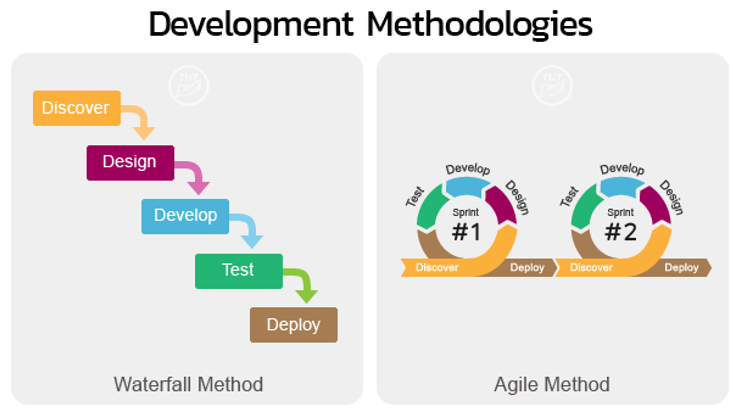
\includegraphics[scale=0.6]{agile}
	\caption{ความแตกต่างระหว่าง Waterfall Method กับ Agile Method}
	\end{figure}
	\item Scrum (สกรัม) คือการนำแนวคิดในการทำงานแบบ Agile (อไจล์) มาปฏิบัติตามขั้นตอนของสกรัม เพื่อระบุปัญหาที่มีความซับซ้อน เปลี่ยนแปลงบ่อย เพื่อให้สามารถส่งมอบผลิตภัณฑ์ที่ตอบสนองต่อการเปลี่ยนแปลงที่เกิดขึ้นได้อย่างรวดเร็ว
ช่วยให้การพัฒนาผลิตภัณฑ์แบบ Agile มีขั้นตอนการการดำเนินงานและผลลัพธ์ที่ชัดเจน โปร่งใส สามารถตรวจสอบประสิทธิภาพของแต่ละขั้นตอนการดำเนินงาน สามารถปรับปรุงและวัดผลการปรับปรุงที่เกิดขึ้นได้
	\item Kanban ที่มาเริ่มต้นมาจากระบบการทำงานของ Toyota ซึ่งประสบความสำเร็จอย่างมากจนทำให้สามารถผลิตรถออกมาได้ไวกว่าคู่แข่งทั่วโลกจนครองตลาดไปได้มาก สำหรับวงการ Software ได้ถูก David J. Anderson จับนำมาปรับปรุงให้เข้ากับ Software Development เพื่อการพัฒนา Software ได้อย่างรวดเร็วที่สุดด้วยเช่นกัน และสุดท้ายถูกนำไปเป็นส่วนหนึ่งของ Lean Software Development รวมไปถึงถูกจัดให้เป็น Agile อีกแบบหนึ่งนอกเหนือไปจาก Scrum อีกด้วย
Kanban มีกฎอยู่แค่ 3 ข้อ 
	\begin{itemize}[leftmargin=0pt,itemindent=3.5cm]
		\item Visualize the workflow – แสดง flow การทำงานของระบบให้ออกมาให้เห็นภาพอย่างชัดเจน สามารถบอกได้ว่าขณะนี้งานไปติดขัดที่จุดไหน 			อย่างไรให้ชัดเจน
		\item Limit Work In Progress (WIP) – จุดหลักของ Kanban เลยคือการ limit งานต่อหนึ่งหน่วยย่อย เช่นงานสำหรับ Development ห้ามถือเกิน	 			2 งานเพื่อป้องกันไม่ให้งาน Overload มากเกินไป และจะทำให้สูญเสียเวลาไปมากกว่าที่ควรจะเป็น
		\item Measure the lead time – วัดผลการทำงานและปรับปรุงให้ดียิ่งขึ้นไปอีก ตรงนี้จะเรียกว่า Cycle time หรือค่าเฉลี่ยที่ Card 1 							อันจะอยู่บนบอร์ดตั้งแต่เริ่มต้นไปจนถึงขึ้นบน production จริง
		\end{itemize}
	\end{itemize}
\end{enumerate}

\subsection{Smart Contract \cite{smartcontract}}
\tab Smart Contract หมายถึง กระบวนการทางดิจิทัล ที่กำหนดขั้นตอนการทำธุรกรรมโดยอัตโนมัติไว้ล่วงหน้า โดยไม่ต้องอาศัยตัวกลาง อย่างเช่น ธนาคาร ซึ่งการสร้าง Smart Contract ที่เป็นระบบอัตโนมัติอย่างเต็มรูปแบบ โดยคู่สัญญาทั้งสองฝ่ายจะมีการตกลงกันก่อนหน้านี้ ถึงขั้นตอน กลไก ในการทำรายการธุรกรรมดังกล่าว ซึ่งการพัฒนานี้ส่งผลกระทบต่อรูปแบบธุรกิจแบบดั้งเดิมของธนาคาร

\subsection{Non-Fungible Token (NFT) \cite{nft}}
\tab NFT ย่อมาจาก Non-Fungible Token เป็นชื่อเรียกของ Cryptocurrency ประเภทหนึ่ง เป็นสินทรัพย์ดิจิทัลที่มีเพียงชิ้นเดียวในโลก ไม่สามารถทำซ้ำหรือคัดลอกได้ ต่อให้มีการก๊อบปี้ไป แต่ต้นฉบับของจริงจะมีอยู่เพียงหนึ่งเดียวเท่านั้น ส่วนโทเคน NFT ก็เป็นเหมือนโฉนด เพื่อแสดงความเป็นเจ้าของสินทรัพย์ชิ้นนั้น

\subsection{Fractional- Non-Fungible Token (F-NFT) \cite{f-nft}}
\tab F-NFT จะเปรียบเหมือนธุรกิจประเภทห้างหุ้นส่วนของกิจการมีแห่งเดียวในโลก มีผู้ร่วมลงทุนอย่างน้อย 2 คนขึ้นไป ทุกคนเป็นเจ้าของกิจการ มีอำนาจในการตัดสินใจร่วมกันในทุก ๆ เรื่อง ดังนั้น F-NFT จึงเป็นเพียงสัดส่วนของ NFT ทั้งหมดที่ถูกแบ่งออกเป็นส่วนย่อย ทำให้ผู้คนจำนวนมากสามารถอ้างสิทธิ์ความเป็นเจ้าของชิ้นส่วนของ NFT เดียวกันได้

\subsection{Asset (สินทรัพย์)  \cite{asset}}
\tab Asset หมายถึง ทรัพยากรที่มีและอยู่ในการควบคุมของกิจการ สินทรัพย์นี้อาจจะเป็นสิ่งที่มีตัวตนหรือไม่มีตัวตนก็ได้ ซึ่งสามารถตีราคามูลค่าเป็นเงินได้ ทรัพยากรดังกล่าวเป็นผล ของ เหตุการณ์ในอดีต ซึ่งกิจการคาดว่าจะได้รับประโยชน์เชิงเศรษฐกิจจากทรัพยากรนั้นในอนาคต

\subsection{Digital Asset (สินทรัพย์ดิจิทัล)  \cite{digital-asset}}
\tab คือ "สิ่งที่มีมูลค่าและเราสามารถเป็นเจ้าของได้ แต่ไม่สามารถแตะต้องได้ทางกายภาพ" สิ่งเหล่านั้นถูกสร้างขึ้นในระบบดิจิทัล และเก็บไว้ในอุปกรณ์อิเล็กทรอนิกส์อย่าง คอมพิวเตอร์ ฮาร์ดแวร์ แล็ปท็อป หรือ อุปกรณ์เก็บข้อมูลต่าง ๆ เป็นต้น

\subsection{พินัยกรรม  \cite{will}}
\tab พินัยกรรม หมายถึง การแสดงเจตนากำหนดการเผื่อตายซึ่งให้มีผลบังคับได้เมื่อถึงแก่ความตาย หรือถ้าเป็นภาษาพูดก็ได้แก่คำสั่งเสียของผู้ตาย โดยในการทำพินัยกรรม กฎหมายกำหนดรูปแบบไว้ 5 แบบด้วยกัน ดังนี้
\begin{enumerate}[label=\thesubsection.\arabic*,leftmargin=0pt,itemindent=2.5cm]
\item พินัยกรรมแบบธรรมดา ผู้ทำต้องทำเป็นหนังสือ คือการพิมพ์ข้อความพินัยกรรมลงในกระดาษ มากน้อยหรือจำนวนกี่แผ่นก็ต้องแล้วแต่เนื้อหาหรือจำนวนทรัพย์สิน   ลงวัน เดือน ปี ที่ทำให้ชัดเจน และผู้ทำต้องลงลายมือชื่อไว้ต่อหน้าพยานอย่างน้อย 2 คน และพยานต้องลงลายมือชื่อรับรองการทำพินัยกรรมในขณะทำด้วย
\item พินัยกรรมแบบเขียนเองทั้งฉบับ ผู้ทำพินัยกรรมจะทำเป็นเอกสารเขียนเองทั้งฉบับก็ได้ แต่ผู้ทำนั้นต้องเขียนพินัยกรรมนั้นด้วยลายมือตนเอง   ลงวัน เดือน ปีที่ทำ และที่สำคัญต้องลงลายมือชื่อผู้ทำด้วย กรณีนี้จะมีพยานมารับรู้การทำพินัยกรรมด้วยหรือไม่มีก็ได้
\item พินัยกรรมแบบเอกสารฝ่ายเมือง เป็นแบบพินัยกรรมที่ต้องอาศัยกระบวนการโดยเฉพาะที่มีเจ้าหน้าที่รัฐเข้ามาเกี่ยวข้อง   ผู้ทำพินัยกรรมต้องไปแจ้งความประสงค์โดยให้ถ้อยคำข้อความของตนแก่เจ้าพนักงานที่เขตหรืออำเภอพร้อมพยานอย่างน้อย 2 คน   เจ้าพนักงานจะอ่านข้อความให้ผู้ทำพินัยกรรมและพยานฟัง เมื่อเห็นว่าถูกต้องครบถ้วนแล้ว ผู้ทำพินัยกรรมพร้อมพยานทั้งสองต้องลงลายมือชื่อไว้   ต่อจากนั้น เจ้าพนักงานจะลงลายมือชื่อ วัน เดือน ปี ที่ทำ พร้อมประทับตราตำแหน่ง
\item พินัยกรรมแบบเอกสารลับ ผู้ทำพินัยกรรมทำพินัยกรรมแล้วปิดผนึก และนำไปที่ที่ทำการอำเภอหรือเขต   ผู้ทำพินัยกรรมต้องลงลายมือชื่อและพยานอีกอย่างน้อย 2 คน และให้ถ้อยคำต่อบุคคลเหล่านั้นว่าเป็นพินัยกรรมของตน   เจ้าหน้าที่จะบันทึกถ้อยคำลง วัน เดือน ปี ที่ทำพินัยกรรมแสดงไว้บนซองและประทับตราตำแหน่งไว้เป็นสำคัญโดยผู้ทำพินัยกรรม   พยานและเจ้าหน้าที่ต้องลงลายมือชื่อไว้หน้าซองตรงที่ปิดผนึก
\item พินัยกรรมแบบทำด้วยวาจา กรณีมีพฤติการณ์พิเศษที่บุคคลไม่สามารถทำพินัยกรรมแบบอื่นที่กล่าวมาข้างต้น เช่น การตกอยู่ในภยันตรายใกล้ความตาย หรืออยู่ในระหว่างสงคราม หรือเกิดมีโรคระบาด   เราสามารถทำพินัยกรรมแบบทำด้วยวาจาก็ได้ โดยผู้ทำพินัยกรรมต้องแสดงเจตนาทำพินัยกรรมต่อหน้าพยานอย่างน้อย 2 คนพร้อมกัน   พยานต้องรับฟังข้อความนั้นแล้วไปแจ้งต่อทางราชการโดยเร็วที่สุด ทั้งยังต้องแจ้งวัน เดือน ปี สถานที่ทำพินัยกรรมและพฤติการณ์พิเศษนั้นด้วย   เจ้าพนักงานต้องจดข้อความที่พยานแจ้งไว้ และพยาน 2 คนนั้นต้องลงลายมือชื่อไว้
\end{enumerate}
ข้อจำกัดและข้อควรระวังในการทำพินัยกรรม
\begin{enumerate}[label=.\arabic*,leftmargin=0pt,itemindent=2.5cm]
\item พินัยกรรมเป็นนิติกรรมที่ต้องทำตามแบบที่กำหนดเท่านั้น
\item ต้องเขียน วัน เดือน ปี ลงลายมือชื่อทั้งผู้ทำพินัยกรรมและผู้ที่เป็นพยาน
\item ผู้ที่เป็นพยานจะต้องไม่เป็นผู้เยาว์หรือผู้หย่อนความสามารถ และต้องไม่เป็นผู้มีส่วนได้เสียในกองมรดกนั้นด้วย
\item ผู้ทำพินัยกรรมต้องมีอายุ 15 ปีบริบูรณ์ขึ้นไป
\item พินัยกรรมควรจะตั้งผู้จัดการมรดกโดยสามารถระบุผู้ทำหน้าที่ผู้จัดการมรดกที่เจ้ามรดกไว้ใจลงในพินัยกรรมไปได้เลย
\item สิทธิ หน้าที่ และความรับผิดชอบ ก็สามารถกำหนดในพินัยกรรมได้
\item ทรัพย์สินที่ระบุในพินัยกรรมต้องเป็นทรัพย์สินหรือสิทธิของผู้ทำพินัยกรรมเท่านั้น ทั้งต้องแยกสินส่วนตัวออกจากสินสมรสด้วย
\item เงินประกันชีวิต เงินบำเหน็จตกทอด เงินมีบำนาญตกทอด เงินฌาปนกิจสงเคราะห์ตกทอด ไม่อาจเป็นมรดกที่ระบุลงในพินัยกรรมได้ เพราะไม่ใช่ทรัพย์ที่เจ้ามรดกมีอยู่ก่อนตาย
\section{งานวิจัยที่เกี่ยวข้อง}
ในส่วนนี้เป็นการสรุปเนื้อหาโดยรวมของงานวิจัยที่เกี่ยวข้องกับการพัฒนาโครงงาน will on blockchain ที่มีการใช้งานในส่วนของ digital asset คือ CryptoWill

\subsection{CryptoWill  \cite{cryptowill}}
โปรเจคนี้ได้อธิบายวิธีการทำระบบ CryptoWill ด้วยการให้ user ทำการเลือกเหรียญที่ต้องการทำ Smart Contract ที่ต้องการส่งให้ทายาทและหลังจากนั้นตัวระบบจะทำการให้กำหนดเวลาของการ contract นี้จะส่งต่อเมื่อไหร่ อย่างเช่น ถ้าตั้ง 2 ปี ผู้ใช้งานจะต้องมาก่อนเวลาที่จะเกิด contract นี้ โดยรูปแบบของการทำจะมีวิธีการดำเนินการดังรูป

\begin{figure}[h]
	\centering
	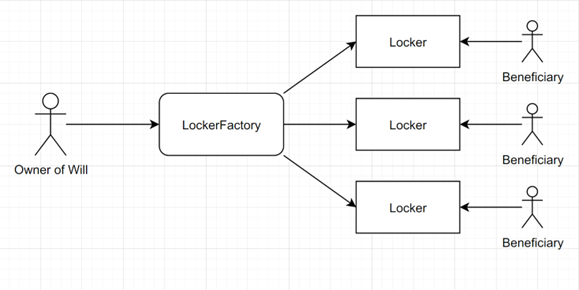
\includegraphics[scale=0.6]{CryptoWill}
	\caption{ภาพแสดงหลักการทำงานของโปรเจค CryptoWill}
\end{figure}

โดยเจ้าของพินัยกรรมจะทำพินัยกรรมและจะเก็บสินทรัพย์ไว้ใน blockchain และหลังจากนั้นจะส่งต่อให้ทายาทไปเมื่อถึงเวลาของพินัยกรรม
\end{enumerate}
\section{เทคนิคและเทคโนโลยีที่ใช้}

\subsection{Ethereum Chain  \cite{eth}} 
\tab Ethereum คือแพลตฟอร์มบน Blockchain Network ที่่ทํางานด้วย Smart Contract มีลักษณะแพลตฟอร์มเป็นรูปแบบ Decentralized Platform แบบ Open Source ทําให้นักพัฒนาสามารถเข้ามาพัฒนา แก้ไข หรือดัดแปลงโค้ดได้ทุกคน พร้อมทั้งกําหนดเงื่อนไขต่าง ๆ สําหรับนําไปใช้งานบน Blockchain โดยมี Smart Contract ดําเนินการและระบบจะทํางานตามเงื่อนไขโปรแกรมที่กําหนดมา ทําให้ผู้ใช้งาน Blockchain ของ Ethereum ทําธุรกรรมได้ โดยไม่ต้องผ่านตัวกลางอื่น

\subsection{GitHub  \cite{github}}
\tab Git คือ Version Control ที่ถูกพัฒนาขึ้นมาเพื่อใช้ใ้นกระบวนการพัฒนาซอฟต์แวร์ คือ ระบบที่ถูกพัฒนาขึ้นมาเพื่อใช้สำหรับการติิดตาม ตรวจสอบ การพัฒนา แก้ไข Source Code ไฟล์ต่าง ๆ ในขั้นตอนการพัฒนา ที่สามารถตรวจสอบ ได้ทุกตัวอักษร ทุกบรรทัด ทุกไฟล์์ที่มีีการแก้ไข และยังมีคุณณลักษณะที่สนับสนุนการทำงานแบบ Agile อีกด้วย จึงทำให้เราสามารถทำงานได้อย่างมีประสิทธิภาพมากยิ่งขึ้น

\subsection{MetaMask \cite{metamask}}
\tab MetaMask หรือ MetaMask Wallet กระเป๋าเงินสินทรัพย์ดิจิทัล เป็น Wallet สำหรับเก็บ Cryptocurrency บนระบบนิเวศของ Ethereum ทุกชนิด ในกลุ่ม ERC-20 ซึ่ง Metamask พัฒนาโดยบริษัท ConsenSys โดยมีผู้ก่อตั้งคือ Joseph Lubin เมื่อปี 2016 (Joseph Lubin ยังเป็นผู้ร่วมก่อตั้ง Ethereum และ เคยยังเคยเป็น Speaker ในงาน Techsauce Global Summit)

\subsection{NestJS \cite{nestjs}}
\tab NestJS เป็น Framework สำหรับ Build Node.js ในฝั่ง Server-side Applications โดยสนันสนุนการทำงานแบบ

	\begin{itemize}[leftmargin=0pt,itemindent=2.5cm]
		\item TypeScript เต็มรูปแบบ
		\item OOP (Object Oriented Programming)
		\item FP (Functional Programming)
		\item FRP (Functional Reactive Programming)
	\end{itemize}

\subsection{Next.js \cite{nextjs}}
\tab Next.js คือ JavaScript webapps framework ถูกสร้างขึ้น on top จาก library ดัง ๆ อย่าง React, Webpack, และ Babel และมีจุดเด่นที่ server-side rendering ที่สามารถ render หน้าเว็บบน server แทนที่จะ render บน browser ได้ จึงทำให้ข้อมูลที่ส่งให้ฝั่ง client นั้นถูก render เสร็จเรียบร้อยแล้ว ทำให้ฝั่ง client สามารถนำไปแสดงผลได้ทันที

\subsection{Solidity \cite{solidity}}
\tab Solidity คือภาษาสำหรับการสร้าง Smart Contract เป็นภาษาที่ได้รับอิทธิพลมาจาก C ++, Python และ JavaScript ที่สำคัญเลยก็คือเป็นภาษาชนิดที่ statically typed และเป็นภาษาแบบ Object Oriented (OO) เพราะว่ามีคุณสมบัติของการสืบทอดและการทำ struct เป็นต้น

\subsection{TypeScript \cite{typescript}}
\tab TypeScript เป็นภาษาโปรแกรมที่รวมความสามารถที่ ES2015 เองมีอยู่ สิ่งที่เพิ่มขึ้นมาคือสนับสนุน Type System รวมถึงคุณสมบัติอื่นๆที่เพิ่มมากขึ้น เช่น Enum และความสามารถที่เพิ่มขึ้นของการโปรแกรมเชิงวัตถุ TypeScript นั้นเป็น transpiler เหมือน Babel นั่นหมายความว่าตัวแปลภาษาของ TypeScript จะแปลโค๊ดที่เราเขียนให้เป็น JavaScript อีกทีนึง จึงมั่นใจได้ว่าผลลัพธ์สุดท้ายจะสามารถใช้งานได้บนเว็บเบราเซอร์ทั่วไป

\subsection{Web3.js \cite{web3js}}
\tab Web3.js เป็น JavaScript API ที่ทําให้ส่วนติดต่อผู้ใช้งานสามารถติดต่อและเรียกใช้ฟังก์ชันจากฝั่งของ Ethereum ได้ โดย Web3.js สามารถส่ง API ไปติดต่อกับฝั่ง Smart Contract ให้สร้าง Transaction สําหรับเรียกใช้ Methods หรือ Get ค่าตัวแปรต่าง ๆ บน Smart Contract ที่อยู่บน Ethereum Blockchain ได้

\subsection{Truffle \cite{truffle}}
\tab Truffle Suite เป็นเครื่องมือ Open source สําหรับพัฒนา Decentralized Application บน Blockchain ที่รองรับ Ethereum virtual machine นอกจากนี้ Truffle Suite ยังเป็น Development Environment, Testing Environment และ Asset Pipeline ที่มุ่งเน้น ให้การทํางานของนักพัฒนาซอฟต์แวร์ง่ายขึ้น และการใช้ Truffle Suite จะมี 

	\begin{itemize}[leftmargin=0pt,itemindent=2.5cm]
		\item Build-in smart contract compiler 
		\item Automated contract testing with Mocha and Chai 
		\item Pipeline ที่สามารถปรับแต่งได้ 
		\item Scriptable deployment and migrations framework 
		\item Network management for deploying to many public and private networks 
		\item Interactive console for direct contract communication 
		\item Instant rebuilding of assets during development 
		\item External script runner that executes scripts within a Truffle environment
	\end{itemize}

\chapter{การออกแบบและวิธีการดำเนินงาน}
\tab เอกสารรายงานบทนี้จะกล่าวถึงระบบการทำงานของโครงงาน รวมถึงแผนภาพต่าง ๆ ที่ใช้อธิบายการทำงานในส่วนต่าง ๆ ของระบบ การออกแบบส่วนติดต่อผู้ใช้งาน (User Interface) ไดอะแกรมของระบบ รวมถึงขั้นตอนและวิธีการดำเนินงาน
\section{ระบบการทำงาน}
\subsection{ภาพรวมของระบบ}
\tab โดยภาพรวมของ Will Chain (Web application) จะประกอบไปด้วย 3 ส่วนหลักดังนี้
	\begin{figure}[h]
		\centering
		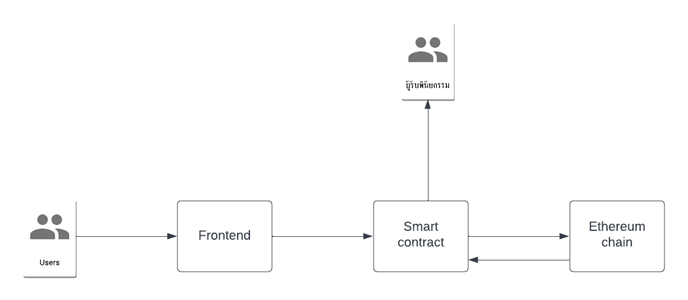
\includegraphics[scale=0.8]{Overall_system}
		\caption{ภาพรวมแสดงการทำงานของระบบ}
	\end{figure}
	\begin{itemize}[leftmargin=0pt,itemindent=2.5cm]
		\item ส่วนติดต่อผู้ใช้งานหรือ Frontend จะเป็นส่วนที่ผู้ใช้งานเห็น และใช้งาน
		\item Smart Contract จะเป็นส่วนที่ควบคุมการทำงานของระบบทั้งหมด โดยที่ผู้ใช้งานจะเข้าใช้งานผ่านทาง Frontend และจะส่งชุดคำสั่งมาเพื่อที่จะสั่งให้ Smart Contract นั้นทำงาน และจะส่งข้อมูลไปเก็บใน Blockchain ต่อไป
		\item Ethereum chain สำหรับเก็บข้อมูลการใช้งานของผู้ใช้งาน
	\end{itemize}

\subsection{User Journey}
	\begin{figure}[h]
		\centering
		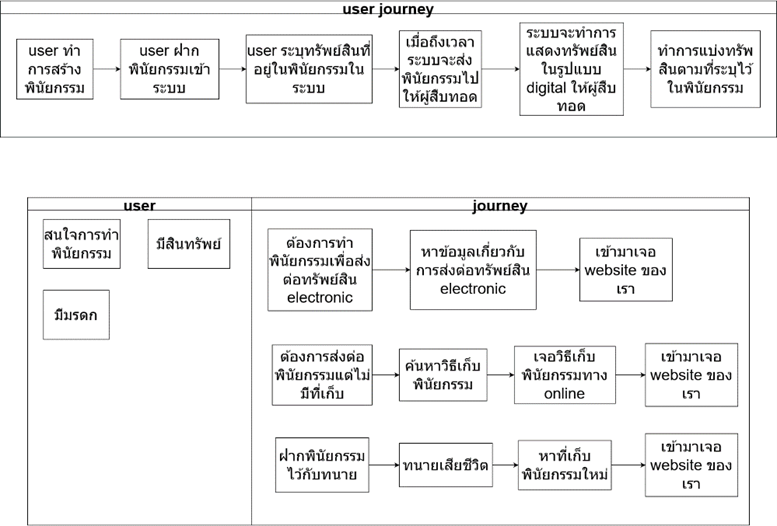
\includegraphics[scale=0.8]{UserJourney}
		\caption{แสดง User Journey}
	\end{figure}
\FloatBarrier
\hfill\\
\hfill\\
\hfill\\
\section{Cryptocurrency Wallet}
\tab ในการออกแบบระบบการทํางานของ Will Chain web application ได้เลือกใช้งาน Cryptocurrency Wallet ที่สามารถเชื่อมต่อกับ
Ethereum chain ได้ เพื่อที่จะทําให้สามารถทดสอบ และใช้งานจริงได้บน Ethereum chain โดย Cryptocurrency Wallet โดยเลือกใช้เป็น Metamask Wallet

\section{Diagram Unified Modelling Language (UML)}
\tab หลังจากได้เขียนความต้องการ และฟังก์ชันแล้ว จึงทำการออกแบบและเขียนแผนภาพไดอะแกรมต่าง ๆ เพื่อให้สามารถเข้าใจระบบการทำงานมากยิ่งขึ้น โดยมีรายละเอียดดังนี้

\subsection{แผนภาพ Use Case Diagram}
	\begin{figure}[!htb]
		\centering
		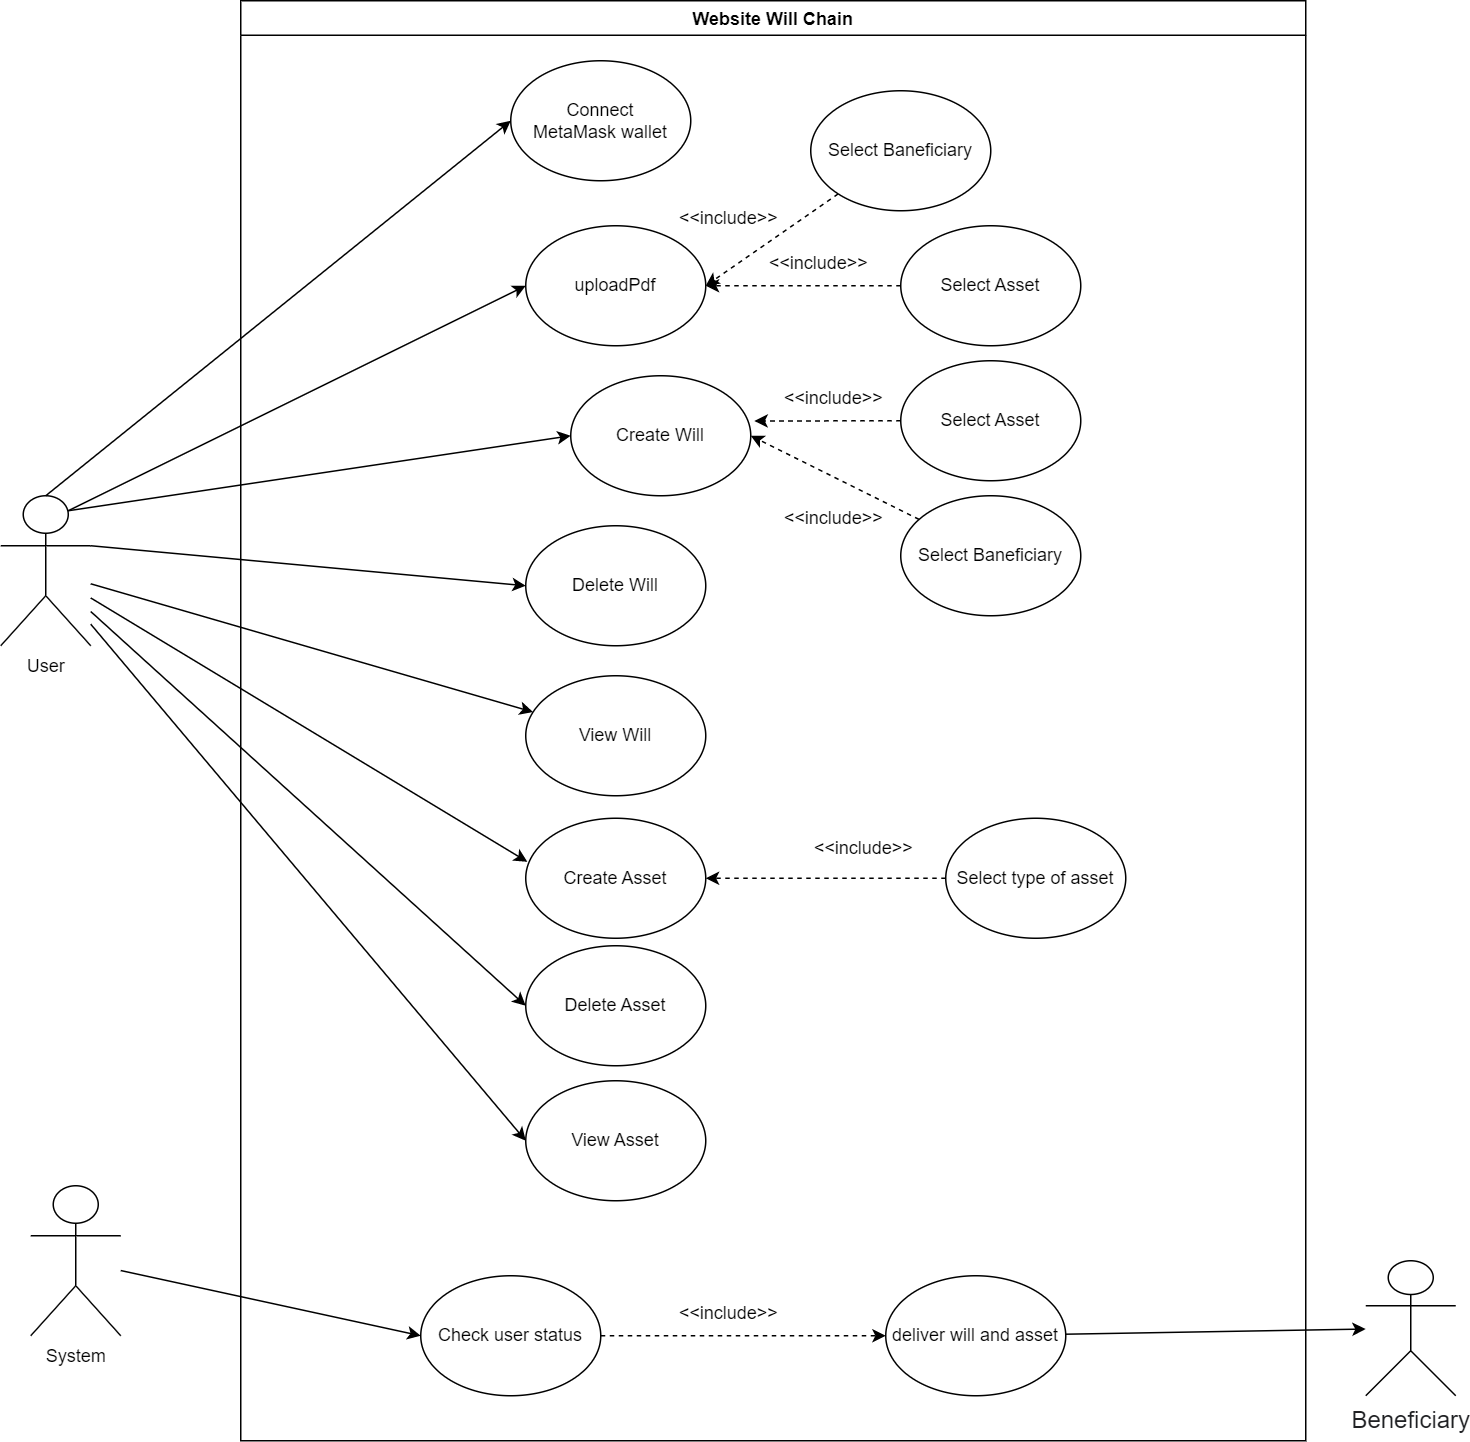
\includegraphics[scale=0.2]{UseCaseDiagram}
		\caption{แสดงการทำงานของระบบทั้งหมด Use Case Diagram}
	\end{figure}
\FloatBarrier
\tab จากรูปแสดง Use Case แสดงการทำงานของระบบทั้งหมดโดยจะมีผู้ใช้งาน (User) ที่ต้องการฝากพินัยกรรมไว้ในระบบทำการใช้งานระบบผ่าน platform ของ WOB โดยผู้ใช้งานจำเป็นต้องเชื่อมต่อกระเป๋าเงินอิเล็กทรอนิกส์ของ meta mask ก่อนหลังจากนั้นจึงจะสามารถ สร้าง,ลบหรือ upload พินัยกรรมพร้อมทั้งมีระบบจัดการทรัพย์สินที่ผู้ใช้แนบไว้พร้อมกับพินัยกรรม และจะมีระบบที่ทำการตรวจสอบสถานะของผู้ใช้งานเพื่นที่จะทำการส่งผ่านพินัยกรรมไปยังผู้รับผลประโยชน์เมื่อถึงเวลา   จากแผนภาพ Use Case Diagram ตามรูปที่ สามารถอธิบายรายละเอียดการทํา งานของแต่ละ Use Case ได้ดังต่อไปนี้ โดยจะกล่าวถึงในหัวข้อ Use Case Narrative ถัดไป
\FloatBarrier
\subsection{Use Case Narrative}
\begin{enumerate}[label=\thesubsection.\arabic*,leftmargin=0pt,itemindent=2.5cm]
\item Use Case Connect Wallet
	\begin{figure}[!htb]
		\centering
		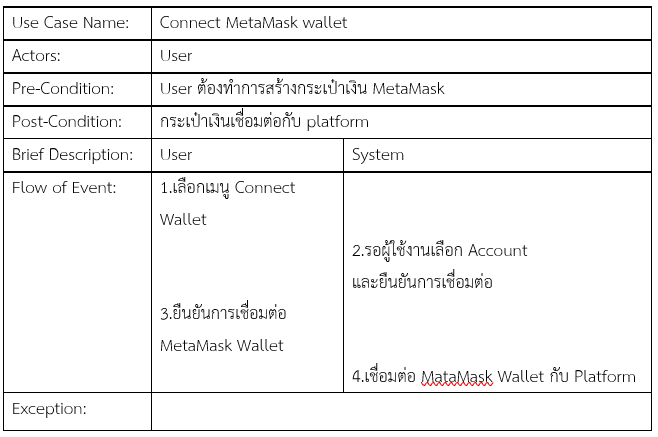
\includegraphics[scale=0.8]{connectwallet}
		\caption{ตารางแสดงรายละเอียดของ Use Case Connect meta mask Wallet}
	\end{figure}
	\FloatBarrier
\item Use Case Upload Will
	\begin{figure}[!htb]
		\centering
		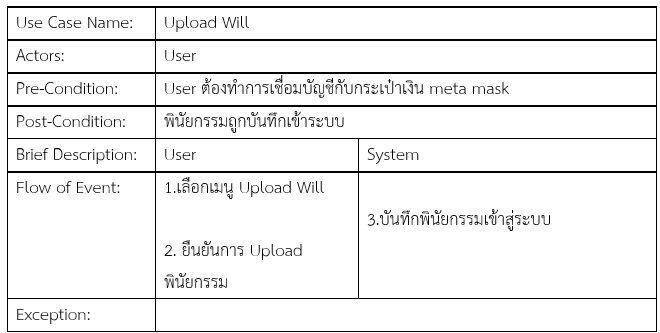
\includegraphics[scale=0.8]{uploadWill}
		\caption{ตารางแสดงรายละเอียดของ Use Case Upload Will}
	\end{figure}
	\FloatBarrier
\item Use Case Create Will
	\begin{figure}[!htb]
		\centering
		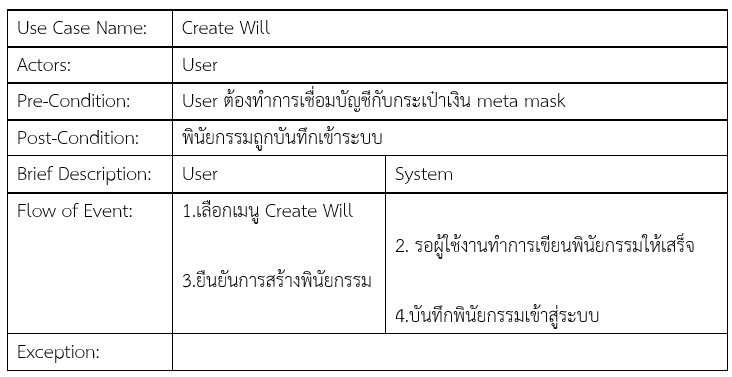
\includegraphics[scale=0.8]{usecasecreatewill}
		\caption{ตารางแสดงรายละเอียดของ Use Case Create Will}
	\end{figure}
	\FloatBarrier
\item Use Case Select Baneficiary
	\begin{figure}[!htb]
		\centering
		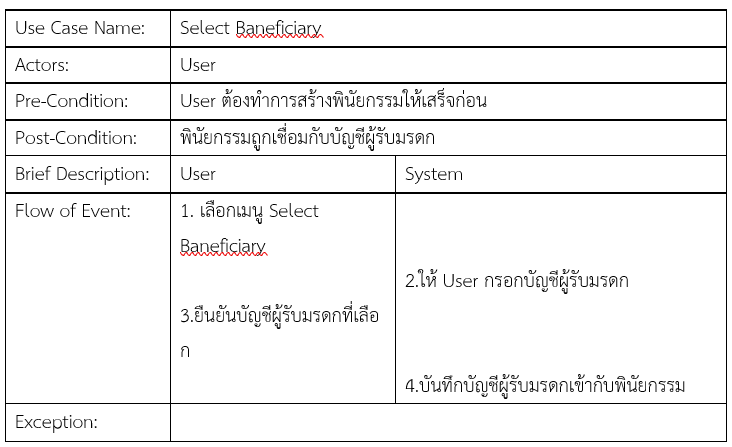
\includegraphics[scale=0.8]{usecaseselectbenaficiary}
		\caption{ตารางแสดงรายละเอียดของ Use Case Select Beneficiary}
	\end{figure}
	\FloatBarrier
\item Use Case Select Asset
	\begin{figure}[!htb]
		\centering
		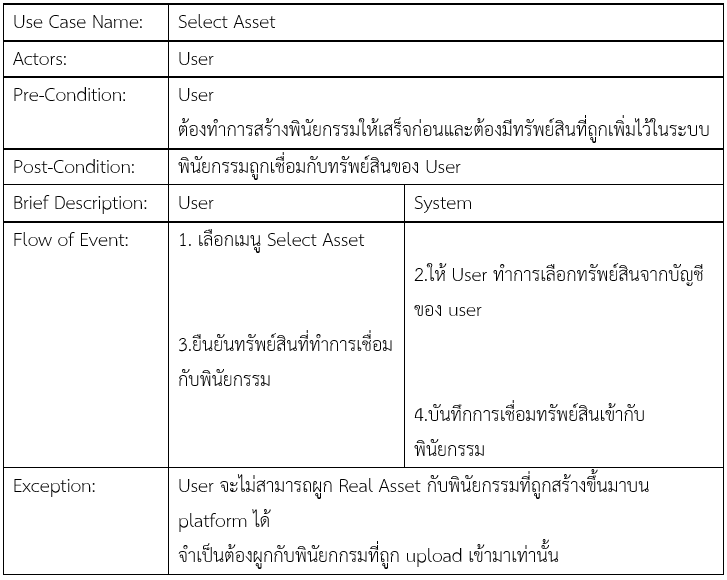
\includegraphics[scale=0.8]{selectAsset}
		\caption{ตารางแสดงรายละเอียดของ Use Case Select Asset}
	\end{figure}
	\FloatBarrier
\item Use Case Delete Will
	\begin{figure}[!htb]
		\centering
		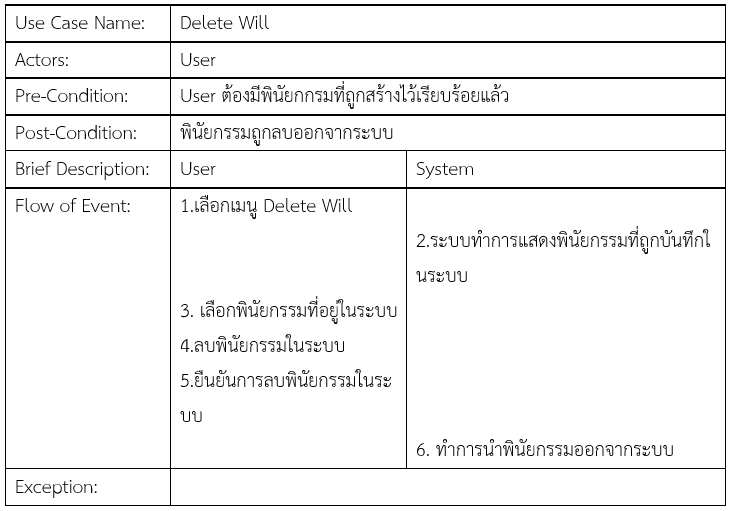
\includegraphics[scale=0.8]{deleteWill}
		\caption{ตารางแสดงรายละเอียดของ Use Case Delete Will}
	\end{figure}
	\FloatBarrier
\item Use Case View Will
	\begin{figure}[!htb]
		\centering
		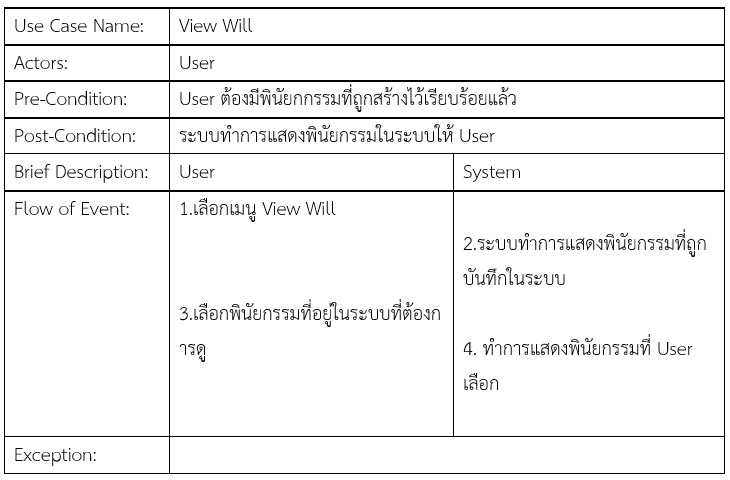
\includegraphics[scale=0.8]{viewWill}
		\caption{ตารางแสดงรายละเอียดของ Use Case View Will}
	\end{figure}
	\FloatBarrier
\item Use Case Create Asset
	\begin{figure}[!htb]
		\centering
		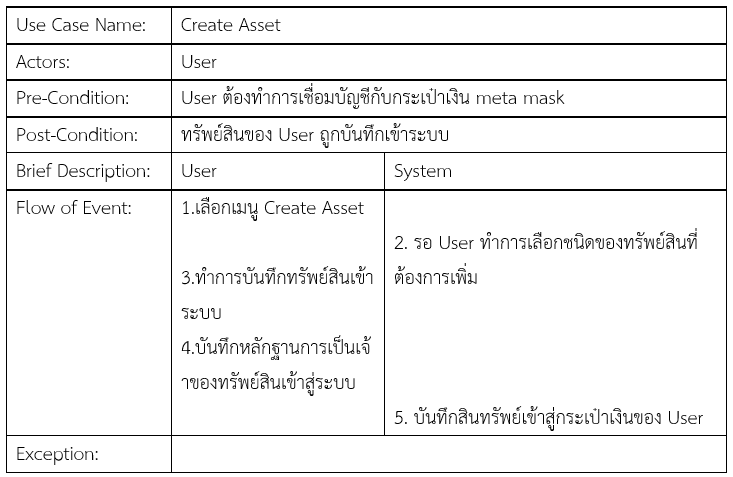
\includegraphics[scale=0.8]{createAsset}
		\caption{ตารางแสดงรายละเอียดของ Use Case Create Assetl}
	\end{figure}
	\FloatBarrier
\item Use Case Delete Asset
	\begin{figure}[!htb]
		\centering
		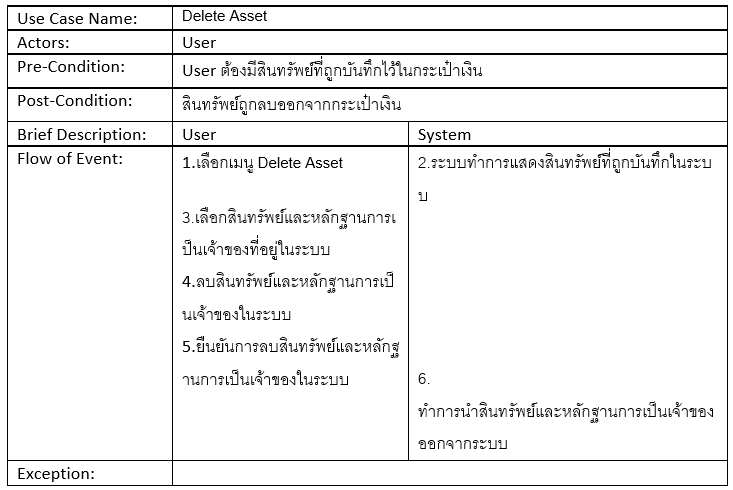
\includegraphics[scale=0.8]{deleteAsset}
		\caption{ตารางแสดงรายละเอียดของ Use Case Delete Asset}
	\end{figure}
	\FloatBarrier
\item Use Case View Asset
	\begin{figure}[!thb]
		\centering
		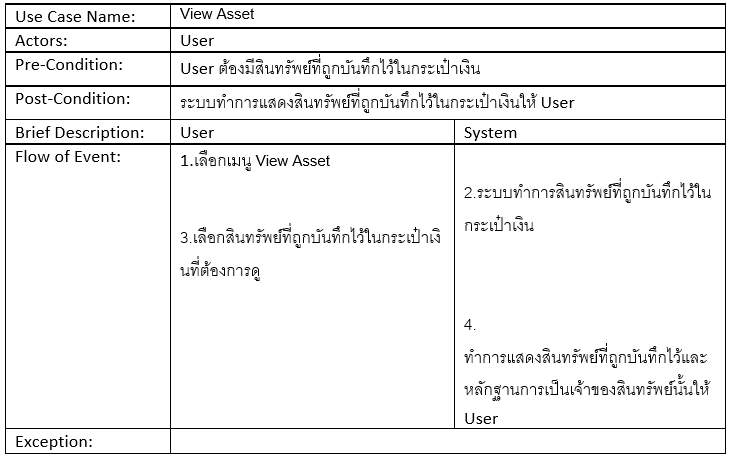
\includegraphics[scale=0.8]{viewAsset}
		\caption{ตารางแสดงรายละเอียดของ Use Case View Asset}
	\end{figure}
	\FloatBarrier
\item Use Case Check user status
	\begin{figure}[!thb]
		\centering
		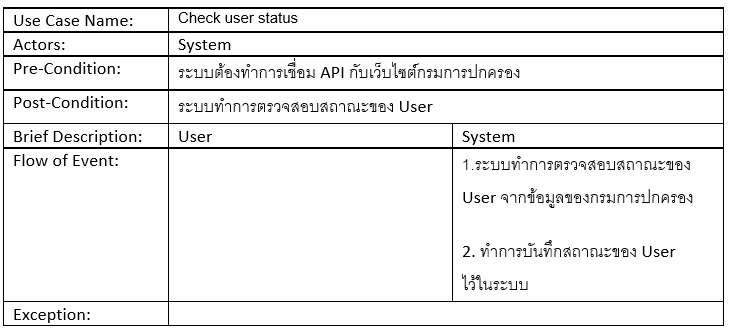
\includegraphics[scale=0.8]{checkUserStatus}
		\caption{ตารางแสดงรายละเอียดของ Use Case Check user status}
	\end{figure}
	\FloatBarrier
\item Use Case deliver will and asset
	\begin{figure}[!thb]
		\centering
		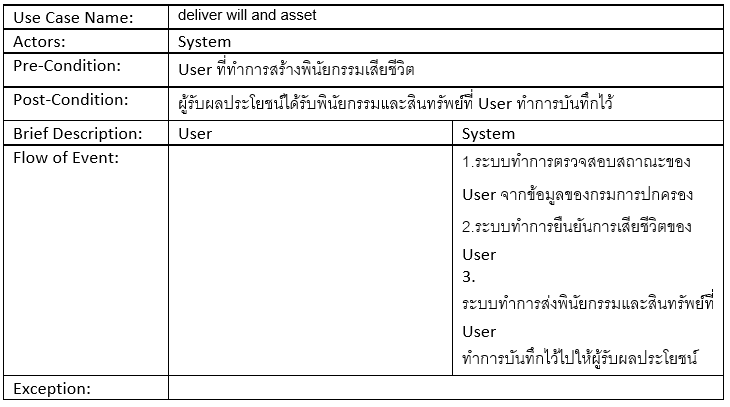
\includegraphics[scale=0.8]{deliverWillAndAsset}
		\caption{ตารางแสดงรายละเอียดของ Use Case deliver will and asset}
	\end{figure}
	\FloatBarrier
\end{enumerate}
\subsection{Class Diagram}

\begin{table}[]
\centering
\caption{ตารางแสดงคำอธิบาย Class Diagram}
\label{tab:my-table}
\resizebox{\textwidth}{!}{%
\begin{tabular}{|l|l|l|}
\hline
\multicolumn{1}{|c|}{ชื่อ Class} & \multicolumn{1}{c|}{หน้าที่}                                                                                                                                                                                                                          & \multicolumn{1}{c|}{ความสัมพันธ์}                                                                    \\ \hline
User                             & \begin{tabular}[c]{@{}l@{}}เก็บข้อมูลของผู้ใช้งาน\\ - แสดงสินทรัพย์ที่ได้รับจากพินัยกรรม\\ - กดรับสินทรัพย์ที่ได้รับจากพินัยกรรมที่ได้รับ\\ - แสดงข้อมูลผู้ใช้งาน (เลขกระเป๋า MetaMask)\\ - แสดงแจ้งเตือนเมื่อได้รับพินัยกรรม\end{tabular}            & - Service Contract                                                                                   \\ \hline
Service Contract                 & \begin{tabular}[c]{@{}l@{}}จัดการ Smart Contract ของระบบ\\ - เช็คสถานะการมีชีวิต\\ - เช็คสถานะพินัยกรรม\\ - เช็คสถานะสินทรัพย์\\ - เช็คเจ้าของพินัยกรรม\\ - เช็คคนที่ได้รับพินัยกรรม\end{tabular}                                                     & \begin{tabular}[c]{@{}l@{}}- Asset\\ - Will\\ - User\end{tabular}                                    \\ \hline
Asset                            & \begin{tabular}[c]{@{}l@{}}เก็บข้อมูลสินทรัพย์\\ - เพิ่มสินทรัพย์\\ - ลบสินทรัพย์\\ - แสดงสินทรัพย์\\ - เช็คชนิดของสินทรัพย์\\ - สร้าง NFT\end{tabular}                                                                                               & \begin{tabular}[c]{@{}l@{}}- Real Asset\\ - Digital Asset\\ - Will\\ - Service Contract\end{tabular} \\ \hline
Real Asset                       & \begin{tabular}[c]{@{}l@{}}เก็บข้อมูลสินทรัพย์ในชีวิตจริง\\ - อัพโหลด pdf\\ - ลบ pdf\\ - เช็คจำนวน pdf\\ - ดูชนิดของสินทรัพย์\end{tabular}                                                                                                            & Inheritace จาก class Asset                                                                           \\ \hline
Digital Asset                    & \begin{tabular}[c]{@{}l@{}}เก็บข้อมูลสินทรัพย์ดิจิทัล\\ - คำนวณจำนวนคงเหลือของสินทรัพย์ดิจิทัล\end{tabular}                                                                                                                                           & Inheritance จาก class Asset                                                                          \\ \hline
Will                             & \begin{tabular}[c]{@{}l@{}}เก็บข้อมูลพินัยกรรม\\ - เพิ่มพินัยกรรม\\ - ลบพินัยกรรม\\ - แสดงพินัยกรรม\\ - เลือกสินทรัพย์\\ - ผูกพินัยกรรมกับสินทรัพย์\\ - เช็คชนิดของพินัยกรรม\\ - สร้าง NFT \\ - อัพโหลด pdf\\ - ลบ pdf\\ - เช็คจำนวน pdf\end{tabular} & \begin{tabular}[c]{@{}l@{}}- Asset \\ - Service Contract\end{tabular}                                \\ \hline
\end{tabular}%
}
\end{table}
\subsection{System Architecture Diagram}
	\begin{figure}[!thb]
		\centering
		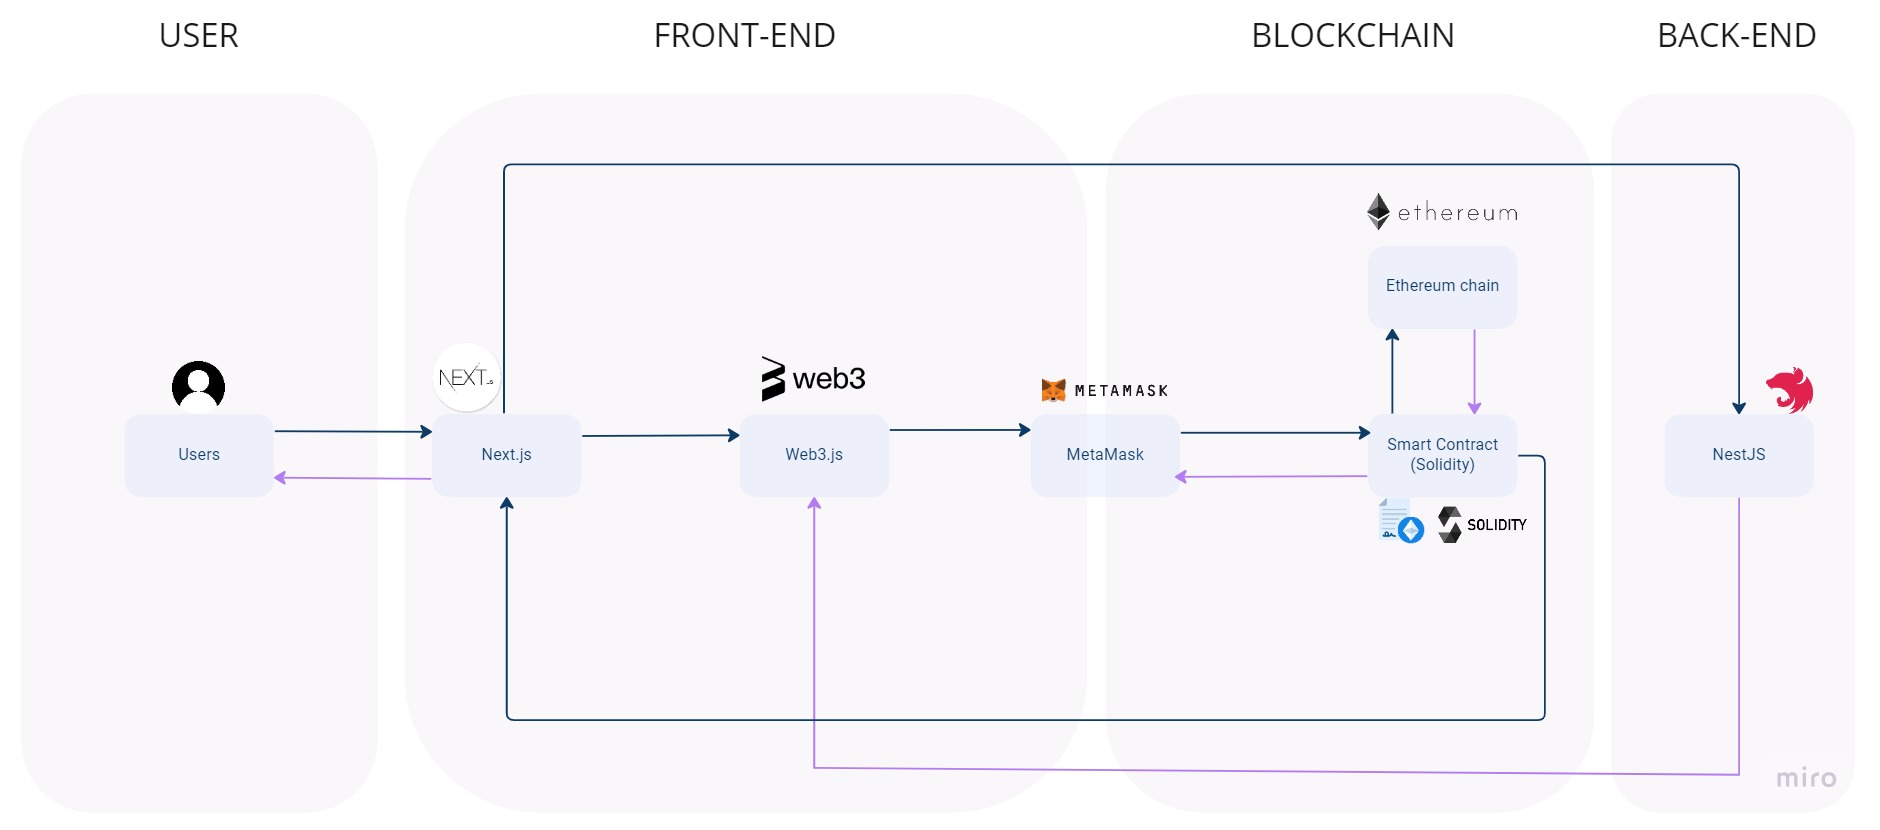
\includegraphics[scale=0.2]{systemArch}
		\caption{แสดงภาพออกแบบสถาปัตยกรรมของระบบ Will Chain}
	\end{figure}
	\FloatBarrier
ระบบของ Will Chain มีส่วนติดต่อกับระบบอื่น ๆ แยกตามประเภทดังนี้ \\
\textbf{Actor ของระบบ}
	\begin{itemize}
		\item User เป็นบุคคลที่ต้องการทำพินัยกรรมของ Will Chain
	\end{itemize}
\textbf{Front-end ของระบบ}
	\begin{itemize}
		\item Next.js จะทำหน้าที่แสดงผล UI ของเว็ปไซต์ Will Chain ในการทำพินัยกรรมต่าง ๆ 
		\item Web3.js จะทำหน้าที่ interact กับ method ต่าง ๆ ใน smart contract
		\item MetaMask จะทำหน้าที่เป็นตัว wallet สำหรับเก็บทรัพย์สินของเราและยังทำหน้าที่เป็นตัว login สำหรับใช้งานในระบบ
	\end{itemize}
\textbf{Blockchain ของระบบ}
	\begin{itemize}
		\item Smart contract จะทำหน้าที่คอยจัดการ transaction ภายใน Ethereum chain
		\item Ethereum chain จะทำหน้าที่เก็บข้อมูล transaction และการทำพินัยกรรมต่าง ๆ ของระบบ
	\end{itemize}
\subsection{Sequence Diagram}
	\begin{enumerate}[label=\thesubsection.\arabic*,leftmargin=0pt,itemindent=2.5cm]
	\item Connect MetaMask
		\begin{figure}[!thb]
			\centering
			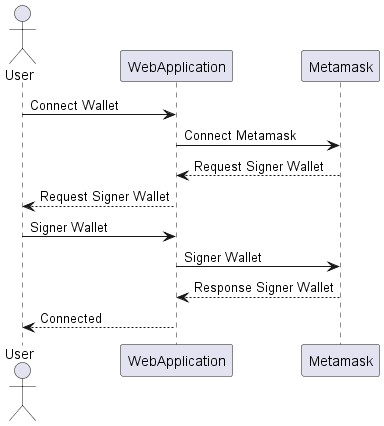
\includegraphics[scale=0.6]{connectMetamaskSeq}
			\caption{แสดง Connect MetaMask Sequence Diagram}
		\end{figure}
		\FloatBarrier
	\tab จากรูป จะเห็นได้ว่าเมื่อผู้ใช้งานทํางาน Connect MetaMask แล้วทางระบบของ Will Chain จะไปเรียกใช้ MetaMask ที่ทําการติดตั้งไว้ใน Web browser ที่ทําการใช้งานอยู่ว่าให้เลือก Account ที่ต้องการทําการเชื่อมต่อ Will on Blockchain ซึ่งหลังจากทําการเลือก Account ที่ต้องการทําการเชื่อมต่อแล้วนั้นทาง Metamask จะให้ถามหา Permission ว่าให้ทําการเชื่อม Account นี้ กับ Will on Blockchain ใช่หรือไม่และหลังจากทําการอนุญาตให้ทําการเชื่อมต่อแล้วจะเสร็จสิ้นการเชื่อม MetaMask กับ Will on Blockchain
	\item Upload Pdf Will
		\begin{figure}[!thb]
			\centering
			\includegraphics[scale=0.6]{uploadPdfWillseq}
			\caption{แสดง Upload Pdf Will Sequence Diagram}
		\end{figure}
		\FloatBarrier
	\tab จากรูป ผู้ใช้เลือกใช้งาน Upload พินัยกรรมที่เขียนด้วยมือระบบจะแสดงฟอร์มที่ใช้สำหรับการ upload โดยหลังจากนั้นจะต้องทำการเลือกสินทรัพย์ที่จะทำการถ่ายทอดไปยังทายาท โดยจะแสดงสินทรัพย์ที่ทำการผูกไว้กับ Smart Contract และหลังจากนั้นจะทำการแสดงผลสินทรัพย์ของ user โดยต่อมาจะทำการเลือกทายาทที่รับผลประโยชน์โดยจะแสดงลิสของทายาทจากการที่ user ทำการเพิ่มไว้ในระบบหลังจากนั้นจึงทำการ upload ไฟล์พินัยกรรมที่เขียนด้วยมือและหลังจาก contract success จะแสดง upload สำเร็จ
	\item Create Will
		\begin{figure}[!thb]
			\centering
			\includegraphics[scale=0.6]{createWillseq}
			\caption{แสดง Create Will Sequence Diagram}
		\end{figure}
		\FloatBarrier
	\tab จากรูป ผู้ใช้เลือกใช้งาน Create Will จะแสดงหน้าจะแสดงฟอร์มสำหรับการทำพินัยกรรมผ่านระบบ ระบบจะให้เลือกสินทรัพย์ดิจิตอลที่ user ทำการเชื่อมต่อไว้กับ Smart Contract โดยหลังจากนั้นจะทำการลิสต์ที่เชื่อมต่อไว้และหลังจากนั้นก็จะทำการเลือกทายาทที่จะรับสินทรัพย์นี้ โดยจะแสดงเป็นลิสต์ของทายาทระบบจทำการเซ็นสัญญาดิจิตอลเพื่อที่เป็นการทำงานคล้ายพินัยกรรมจริง ๆ สุดท้ายระบบจะทำการ confirm เพื่อเป็นการเสร็จการทำพินัยกรรมในระบบ
	\item Delete Will
		\begin{figure}[!thb]
			\centering
			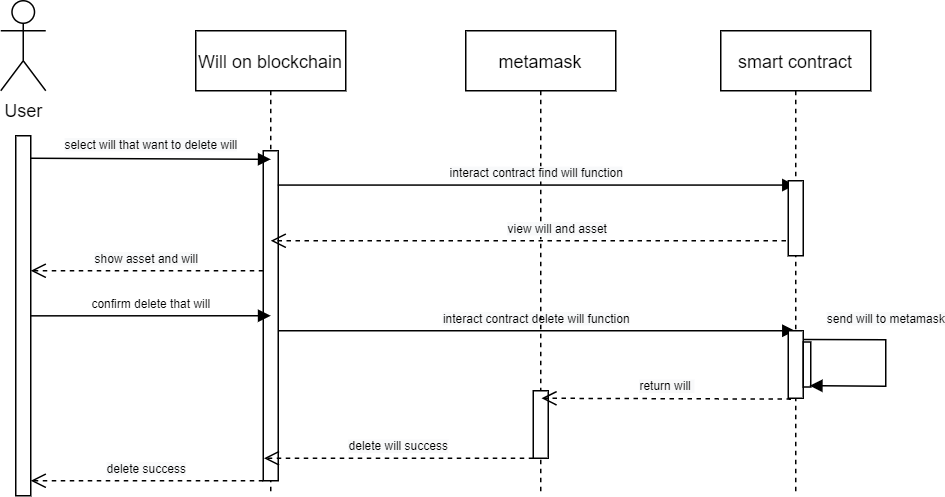
\includegraphics[scale=0.6]{deleteWillseq}
			\caption{แสดง Delete Will Sequence Diagram}
		\end{figure}
		\FloatBarrier
	\tab จากรูป ผู้ใช้ต้องการทำการลบ พินัยกรรมที่มีอยู่ในระบบ โดยระบบจะทำการหาพินัยกรรมที่การที่จะลบภายใน blockchain โดยระบบจะแสดงสินทรัพย์ที่ทำการเชื่อมไว้กับพินัยกรรมและหลังจากนั้นผู้ใช้ทำการยืนยันว่าจะลบระบบจะทำการลบพินัยกรรมที่เชื่อมไว้กับ Smart Contract โดยหลังจากนั้นจะทำการส่งพินัยกรรมที่มีสินทรัพย์อยู่ด้วยไปที่ MetaMask โดยหลังจากที่ MetaMask ได้รับสินทรัพย์จะแสดงเตือนไปที่ผู้ใช้ว่าลบพินัยกรรมสำเร็จ
	\item View Will
		\begin{figure}[!thb]
			\centering
			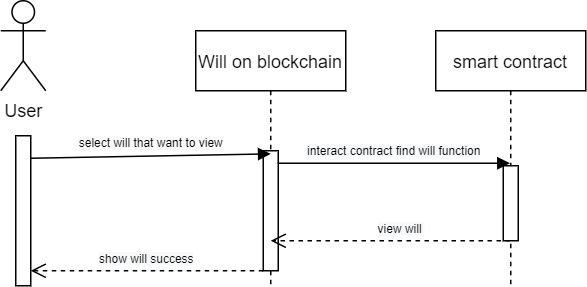
\includegraphics[scale=0.6]{viewWillseq}
			\caption{แสดง View Will Sequence Diagram}
		\end{figure}
		\FloatBarrier
	\tab จากรูป ผู้ใช้ทำการเลือกพินัยกรรมที่ต้องการจะแสดงโดยจะทำการเรียกใช้ฟังก์ชั่นเพื่อหาพินัยกรรมโดยหลังจากที่ Smart Contract ส่งข้อมูลของพินัยกรรมมา ตัวระบบจะทำการแสดงรายละเอียดพินัยกรรม
	\item View Real Asset
		\begin{figure}[!thb]
			\centering
			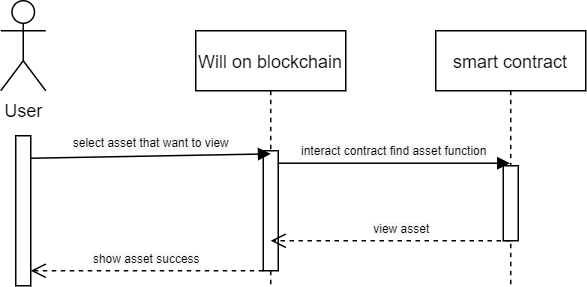
\includegraphics[scale=0.6]{viewRealAssetseq}
			\caption{แสดง View Asset Sequence Diagram}
		\end{figure}
		\FloatBarrier
	\tab จากรูป ผู้ใช้ต้องการดูสินทรัพย์ที่เชื่อมอยู่ Smart Contract โดยจะทำการเรียกใช้ฟังก์ชั่นเพื่อหาพินัยกรรมโดยหลังจากที่ Smart Contract ส่งข้อมูลของสินทรัพย์มา ตัวระบบจะทำการแสดงรายละเอียดสินทรัพย์นั้น
	\item Delete Asset
		\begin{figure}[!thb]
			\centering
			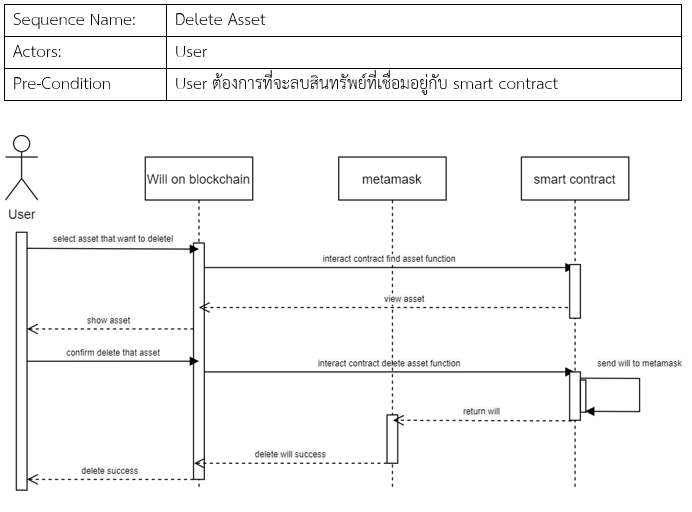
\includegraphics[scale=0.6]{deleteAssetseq}
			\caption{แสดง Delete Asset Sequence Diagram}
		\end{figure}
		\FloatBarrier
	\tab จากรูป ผู้ใช้ต้องการที่จะลบสินทรัพย์ โดยจะทำการเรียกใช้ฟังก์ชั่นเพื่อหาพินัยกรรมโดยหลังจากที่ Smart Contract ส่งข้อมูลของสินทรัพย์มา ตัวระบบจะทำการแสดงรายละเอียดสินทรัพย์นั้นและระบบจะทำการให้ยืนยันการลบสินทรัพย์ออกจาก smart contract และหลังจากนั้นสินทรัพย์จะถูกโอนไปที่ MetaMask ของผู้ใช้และหลังจากนั้นจะแสดงการลบสำเร็จ
	\item Check Status Death
		\begin{figure}[!thb]
			\centering
			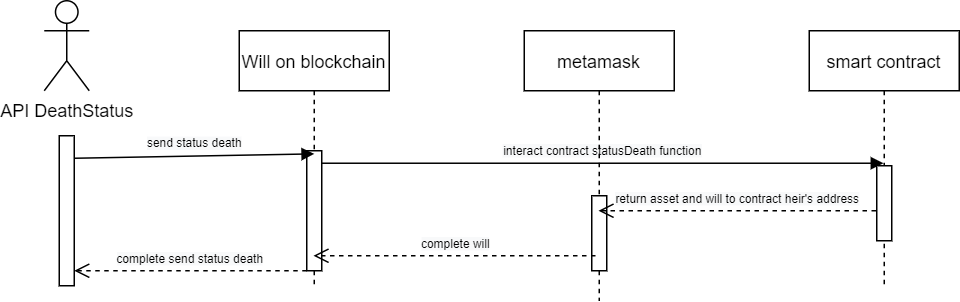
\includegraphics[scale=0.6]{checkStatusDeathseq}
			\caption{แสดง Check Status Death Sequence Diagram}
		\end{figure}
		\FloatBarrier
	\tab จากรูป API Death Status จะทำการส่งสถานะการเสียชีวิตไปที่ระบบ will on blockchain หลังจากนั้นจะส่งไปที่ Smart Contract โดยถ้าสถานะเป็นจริง จะทำการส่งสินทรัพย์และพินัยกรรมไปที่กระเป๋าพินัยกรรมของทายาท
	\item Create Real Asset
		\begin{figure}[!thb]
			\centering
			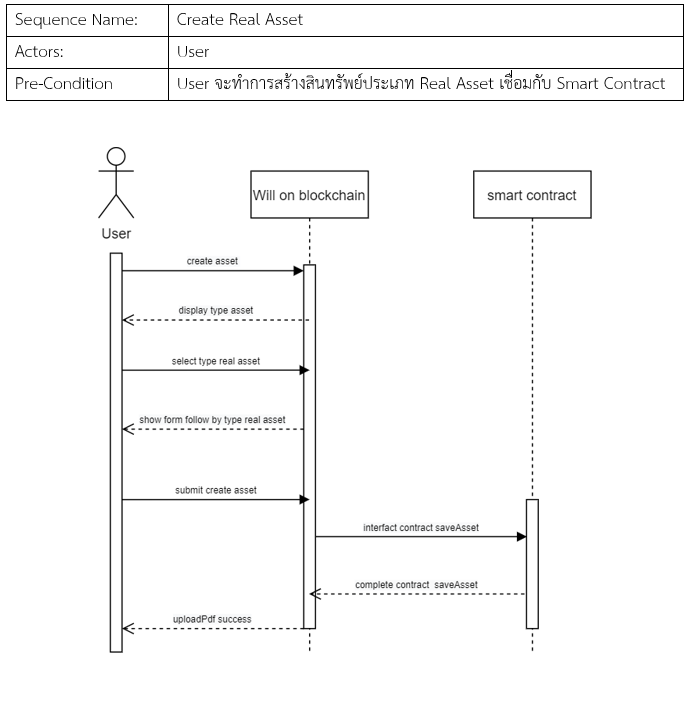
\includegraphics[scale=0.6]{createRealAssetseq}
			\caption{แสดง Create Real Asset Sequence Diagram}
		\end{figure}
		\FloatBarrier
	\tab จากรูป ผู้ใช้งานต้องการทำจะเพิ่มสินทรัพย์ประเภทที่จับต้องได้อยู่จริง ระบบจะทำการแสดงประเภทของสินทรัพย์โดยผู้ใช้งานเลือกประเภทและจะทำการกรอกข้อมูลสินทรัพย์ตามประเภทของสินทรัพย์ที่เลือกหลังจากกรอกเสร็จสิ้นจะทำการ submit เพื่อยืนยันว่าจะเก็บพินัยกรรมไว้ที่ blockchain
	\item Create Digital Asset
		\begin{figure}[!thb]
			\centering
			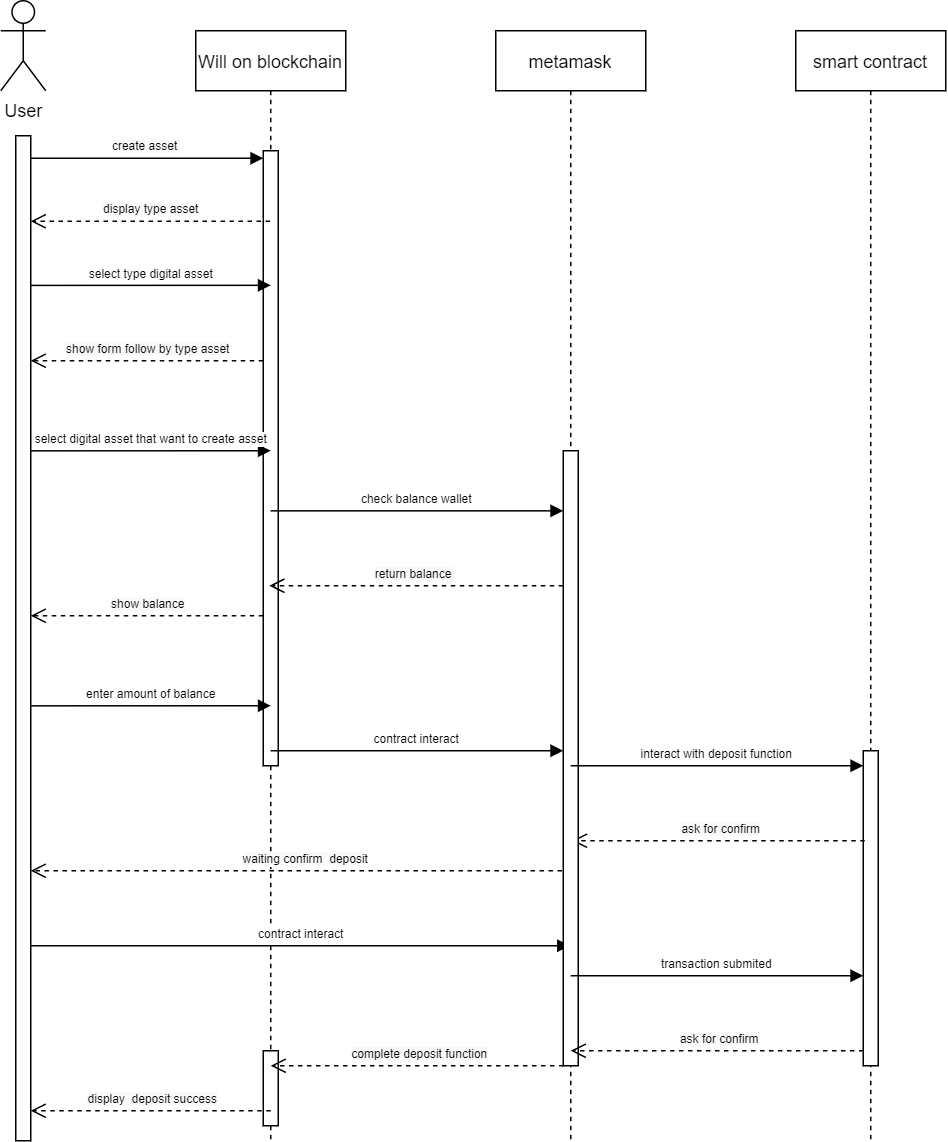
\includegraphics[scale=0.6]{createDigitalAssetseq}
			\caption{แสดง Create Digital Asset Sequence Diagram}
		\end{figure}
		\FloatBarrier
	\tab จากรูป ผู้ใช้จะสร้างสินทรัพย์ประเภทดิจิตอล ระบบ Will on blockchain จะแสดงประเภทของสินทรัพย์ดิจิตอล ผู้ใช้จะทำการเลือกประเภทของสินทรัพย์ โดยระบบจะแสดงฟอร์มสำหรับการสร้างสินทรัพย์ดิจิตอลหลังจากเลือกประเภทเหรียญก็จะทำการใส่สินทรัพย์ที่เหลืออยู่ และจึงจะทำการเก็บไว้ที่ blockchain โดยหลังจากยืนยันระบบจะแสดงว่าทำการสร้างสินทรัพย์ดิจิตอลเสร็จสิ้น
	\item Calm Asset
		\begin{figure}[!thb]
			\centering
			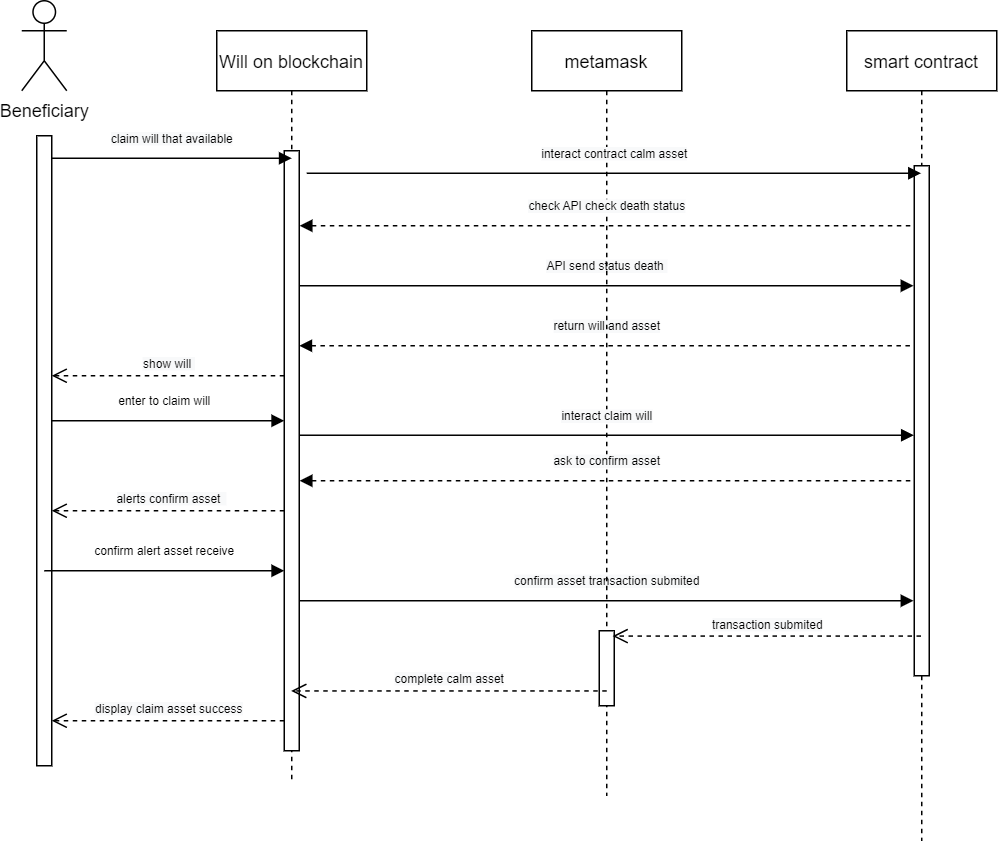
\includegraphics[scale=0.6]{calmAssetseq}
			\caption{แสดง Clailm Asset Sequence Diagram}
		\end{figure}
		\FloatBarrier
	\tab จากรูป ทายาทจะรับสินทรัพย์ที่ได้รับจากการเขียนพินัยกรรมโดยจะทำการเช็คไปที่ Smart Contract ถ้า API check status death ส่งสถานะมาว่าเสียชีวิต ระบบจะทำการแสดงพินัยกรรม ต่อมาผู้ใช้จะทำการ enter เพื่อที่จะทำการรับพินัยกรรมหลังจากนั้น Smart Contract ส่งแจ้งเตือนว่าให้ทำการยืนยันอีกรอบเพื่อที่ระบบจะทำการนำสินทรัพย์ไปเก็บไว้ที่ MetaMask ของผู้ใช้หลังจากทำรายการรับสินทรัพย์เสร็จแล้วระบบจะแสดงผลลัพท์รับสินทรัพย์เสร็จสิ้น
	\end{enumerate}
\section{ส่วนติดต่อผู้ใช้งาน (User Interface)}
\tab การออกแบบส่วนติดต่อผู้ใช้งาน โดยการออกแบบ Will Chain ได้คำนึงถึงการใช้งานของผู้ใช้งาน 
	
\subsection{ออกแบบการทดสอบ}
\section{อัลกอริทึมในการประมวลผลข้อความ}
\subsection{อัลกอริทึม I}

% Can define this in the preamble..
You can place the figure and refer to it as รูปที่~\ref{fig:model2}.
The figure and table numbering will be run and updated automatically when you add/remove tables/figures from the document.

\begin{figure}[!h]\centering
\setlength{\fboxrule}{0.2mm} % can define this in the preamble
\setlength{\fboxsep}{1cm}
\fbox{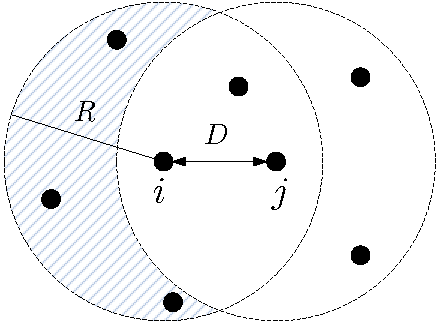
\includegraphics[width=5cm]{./model2.pdf}}
\caption{The network model}\label{fig:model2}
\end{figure}

 
\subsection{อัลกอริทึม I}
Add more subsections as you want.


\section{เครื่องมือที่ใช้ในการพัฒนา}

%%%%%%%%%%%%%%%%%%%%%%%%%%%%%%%%%%%%%%%%%%%%%%%%%%%%%55
%%%%%%%%%%%%%%%%%%%%%%%%%%%%%%%%%%%%%%%%%%%%%%%%%%%%%
%%%%%%%%%%%%%%%%%%%%%%%%%%%%%%%%%%%%%%%%%%%%%%%%%%%%%
\chapter{วิธีการดำเนินงาน}

Explain the design (how you plan to implement your work) of your project. Adjust the section titles below to suit the types of your work. Detailed physical design like circuits and source codes should be placed in the appendix.

\section{ข้อกำหนดและความต้องการของระบบ}

\section{สถาปัตยกรรมระบบ}

\begin{table}[!h]
\centering
\caption{test table x1}\label{tbl:symbols}
\begin{tabular}{@{}p{0.07\textwidth}|p{0.7\textwidth}p{0.1\textwidth}}\hline
\multicolumn{2}{l}{\textbf{SYMBOL}}  & \textbf{UNIT} \\ \hline 
$\alpha$ & Test variable\hfill & m$^2$ \\
$\lambda$ & Interarrival rate\hfill &  jobs/second\\
$\mu$ & Service rate\hfill & jobs/second \\ \hline
\end{tabular}
%\begin{tabular}{c|c} \hline
% $\alpha$ & $\beta$ \\ \hline
% $\delta$ & $\mu$ \\ \hline
%\end{tabular}
\end{table}



\section{Hardware Module 1}
\subsection{Component 1}
\subsection{Logical Circuit Diagram}

\section{Hardware Module 2}
\subsection{Component 1}
\subsection{Component 2}

\section{Path Finding Algorithm}

\section{Database Design}

\section{UML Design}

\section{GUI Design}

\section{การออกแบบการทดลอง}
\subsection{ตัวชี้วัดและปัจจัยที่ศึกษา}
\subsection{รูปแบบการเก็บข้อมูล}




%%%%%%%%%%%%%%%%%%%%%%%%%%%%%%%%%%%%%%%%%%%%%%%%%%%%%%%%%%%%%%
%%%%%%%%%%%%%%%%%%%% Experiments %%%%%%%%%%%%%%%%%%%%%%%%%%%%%
%%%%%%%%%%%%%%%%%%%%%%%%%%%%%%%%%%%%%%%%%%%%%%%%%%%%%%%%%%%%%%%
\chapter{ผลการดำเนินงาน}

You can title this chapter as \textbf{Preliminary Results} ผลการดำเนินงานเบื้องต้น or \textbf{Work Progress} ความก้าวหน้าโครงงาน for the progress reports. Present implementation or experimental results here and discuss them.
ใส่เฉพาะหัวข้อที่เกี่ยวข้องกับงานที่ทำ 

\section{ประสิทฺธิภาพการทำงานของระบบ} 
\section{ความพึงพอใจการใช้งาน}
\section{การวิเคราะห์ข้อมูลและผลการทดลอง}

%%%%%%%%%%%%%%%%%%%%%%%%%%%%%%%%%%%%%%%%%%%%%%%%%%%%%%%%%%%%%%%
%%%%%%%%%%%%%%%%%%%% Conclusions %%%%%%%%%%%%%%%%%%%%%%%%%%%%%
%%%%%%%%%%%%%%%%%%%%%%%%%%%%%%%%%%%%%%%%%%%%%%%%%%%%%%%%%%%%%%%
\chapter{บทสรุป}

This chapter is optional for proposal and progress reports but 
is required for the final report.

\section{สรุปผลโครงงาน}
สรุปว่าโครงงานบรรลุตามวัตถุประสงค์ที่ตั้งไว้หรือไม่ อย่างไร 

\section{ปัญหาที่พบและการแก้ไข}
State your problems and how you fixed them.

\section{ข้อจำกัดและข้อเสนอแนะ}
ข้อจำกัดของโครงงาน What could be done in the future to make your projects better.

%%%%%%%%%%%%%%%%%%%%%%%%%%%%%%%%%%%%%%%%%%%%%%%%%%%%%%%%%%%%%%%
%%%%%%%%%%%%%%%%%%%% Bibliography %%%%%%%%%%%%%%%%%%%%%%%%%%%%%
%%%%%%%%%%%%%%%%%%%%%%%%%%%%%%%%%%%%%%%%%%%%%%%%%%%%%%%%%%%%%%%

%%%% Comment this in your report to show only references you have
%%%% cited. Otherwise, all the references below will be shown.
%\nocite{*}
%% Use the kmutt.bst for bibtex bibliography style 
%% You must have cpe.bib and string.bib in your current directory.
%% You may go to file .bbl to manually edit the bib items.

\makeatletter
\g@addto@macro{\UrlBreaks}{\UrlOrds}
\makeatother

\bibliographystyle{kmutt}
\bibliography{string,cpe}

%%%%%%%%%%%%%%%%%%%%%%%%%%%%%%%%%%%%%%%%%%%%%%%%%%%%%%%%%%%%%%%
%%%%%%%%%%%%%%%%%%%%%%%% Appendix %%%%%%%%%%%%%%%%%%%%%%%%%%%%%
%%%%%%%%%%%%%%%%%%%%%%%%%%%%%%%%%%%%%%%%%%%%%%%%%%%%%%%%%%%%%%%
\appendix{ชื่อภาคผนวกที่ 1}
\noindent{\large\bf ใส่หัวข้อตามความเหมาะสม} \\

This is where you put hardware circuit diagrams, detailed experimental data in tables or source codes, etc.. \\ \bigskip



This appendix describes two static allocation methods for fGn (or fBm)
traffic. Here, $\lambda$ and $C$ are respectively the traffic arrival
rate and the service rate per dimensionless time step. Their unit are
converted to a physical time unit by multiplying the step size
$\Delta$. For a fBm self-similar traffic source,
Norros~\cite{norros95} provides its EB as
\begin{equation}\label{eq:norros}
  C = \lambda + (\kappa(H)\sqrt{-2\ln\epsilon})^{1/H}a^{1/(2H)}x^{-(1-H)/H}\lambda^{1/(2H)}
\end{equation}
where $\kappa(H) = H^H(1-H)^{(1-H)}$. Simplicity in the calculation is
the attractive feature of (\ref{eq:norros}).

The MVA technique developed in~\cite{kim01} so far provides the most
accurate estimation of the loss probability compared to previous
bandwidth allocation techniques according to simulation results.
Consider a discrete-time queueing system with constant service rate
$C$ and input process $\lambda_n$ with $\mathbb{E}\{\lambda_n\} =
\lambda$ and $\mathrm{Var}\{\lambda_n\} = \sigma^2$.  Define $X_n \equiv
\sum_{k=1}^n \lambda_k - Cn$.  The loss probability due to the MVA
approach is given by
\begin{equation}\label{eq:loss_mva}
  \varepsilon \approx \alpha e^{-m_x/2}
\end{equation}
where
\begin{equation}\label{eq:mx}
m_x = \min_{n \geq 0} \frac{((C-\lambda)n + B)^2}{\mathrm{Var}\{X_n\}} =
\frac{((C-\lambda)n^\ast + B)^2}{\mathrm{Var}\{X_{n^{\ast}}\}}
\end{equation} 
and 
\begin{equation}\label{eq:alpha}
  \alpha =
  \frac{1}{\lambda\sqrt{2\pi\sigma^2}}\exp\left(\frac{(C-\lambda)^2}{2\sigma^2}\right)
  \int_C^\infty (r-C)\exp\left(\frac{(r-\lambda)^2}{2\sigma^2}\right)\, dr
\end{equation}

For a given $\varepsilon$, we numerically solve for $C$ that satisfies
(\ref{eq:loss_mva}). Any search algorithm can be used to do the task.
Here, the bisection method is used.  

Next, we show how $\mathrm{Var}\{X_n\}$ can be determined.  Let
$C_{\lambda}(l)$ be the autocovariance function of $\lambda_n$.  The
MVA technique basically approximates the input process $\lambda_n$
with a Gaussian process, which allows $\mathrm{Var}\{X_n\}$ to be
represented by the autocovariance function.  In particular, the
variance of $X_n$ can be expressed in terms of $C_{\lambda}(l)$ as
\begin{equation}
  \mathrm{Var}\{X_n\} = nC_{\lambda}(0) + 2\sum_{l=1}^{n-1} (n-l)C_{\lambda}(l)
\end{equation} 
Therefore, $C_{\lambda}(l)$ must be known in the MVA technique, either
by assuming specific traffic models or by off-line analysis in case of
traces.  In most practical situations, $C_{\lambda}(l)$ will not be
known in advance, and an on-line measurement algorithm developed
in~\cite{eun01} is required to jointly determine both $n^\ast$ and
$m_x$. For fGn traffic, $\mathrm{Var}\{X_n\}$ is equal to $\sigma^2
n^{2H}$, where $\sigma^2 = \mathrm{Var}\{\lambda_n\}$, and we can find
the $n^\ast$ that minimizes (\ref{eq:mx}) directly. Although $\lambda$
can be easily measured, it is not the case for $\sigma^2$ and $H$.
Consequently, the MVA technique suffers from the need of prior
knowledge traffic parameters.


%%%%%%%%%%%%%%%%%%%%%%%%%%%%%%%%%%%%%%%%%%%%%%%%%%%%%%%%%%
%%%%%%%%%%%%%%% The 2nd appendix %%%%%%%%%%%%%%%%%%%%%%%%%%
%%%%%%%%%%%%%%%%%%%%%%%%%%%%%%%%%%%%%%%%%%%%%%%%%%%%%%%%%%
\appendix{ชื่อภาคผนวกที่ 2}
\noindent{\large\bf ใส่หัวข้อตามความเหมาะสม} \\

Next, we show how $\mathrm{Var}\{X_n\}$ can be determined.  Let
$C_{\lambda}(l)$ be the autocovariance function of $\lambda_n$.  The
MVA technique basically approximates the input process $\lambda_n$
with a Gaussian process, which allows $\mathrm{Var}\{X_n\}$ to be
represented by the autocovariance function.  In particular, the
variance of $X_n$ can be expressed in terms of $C_{\lambda}(l)$ as
\begin{equation}
  \mathrm{Var}\{X_n\} = nC_{\lambda}(0) + 2\sum_{l=1}^{n-1} (n-l)C_{\lambda}(l)
\end{equation} 

\noindent{\large\bf Add more topic as you need} \\

Therefore, $C_{\lambda}(l)$ must be known in the MVA technique, either
by assuming specific traffic models or by off-line analysis in case of
traces.  In most practical situations, $C_{\lambda}(l)$ will not be
known in advance, and an on-line measurement algorithm developed
in~\cite{eun01} is required to jointly determine both $n^\ast$ and
$m_x$. For fGn traffic, $\mathrm{Var}\{X_n\}$ is equal to $\sigma^2
n^{2H}$, where $\sigma^2 = \mathrm{Var}\{\lambda_n\}$, and we can find
the $n^\ast$ that minimizes (\ref{eq:mx}) directly. Although $\lambda$
can be easily measured, it is not the case for $\sigma^2$ and $H$.
Consequently, the MVA technique suffers from the need of prior
knowledge traffic parameters. 





\end{document}
